\documentclass[]{article}
\usepackage{lmodern}
\usepackage{amssymb,amsmath}
\usepackage{ifxetex,ifluatex}
\usepackage{fixltx2e} % provides \textsubscript
\ifnum 0\ifxetex 1\fi\ifluatex 1\fi=0 % if pdftex
  \usepackage[T1]{fontenc}
  \usepackage[utf8]{inputenc}
\else % if luatex or xelatex
  \ifxetex
    \usepackage{mathspec}
  \else
    \usepackage{fontspec}
  \fi
  \defaultfontfeatures{Ligatures=TeX,Scale=MatchLowercase}
\fi
% use upquote if available, for straight quotes in verbatim environments
\IfFileExists{upquote.sty}{\usepackage{upquote}}{}
% use microtype if available
\IfFileExists{microtype.sty}{%
\usepackage{microtype}
\UseMicrotypeSet[protrusion]{basicmath} % disable protrusion for tt fonts
}{}
\usepackage[margin=1in]{geometry}
\usepackage{hyperref}
\hypersetup{unicode=true,
            pdftitle={Dynamic Document for Fiscal Impacts of Deworming},
            pdfborder={0 0 0},
            breaklinks=true}
\urlstyle{same}  % don't use monospace font for urls
\usepackage{color}
\usepackage{fancyvrb}
\newcommand{\VerbBar}{|}
\newcommand{\VERB}{\Verb[commandchars=\\\{\}]}
\DefineVerbatimEnvironment{Highlighting}{Verbatim}{commandchars=\\\{\}}
% Add ',fontsize=\small' for more characters per line
\usepackage{framed}
\definecolor{shadecolor}{RGB}{248,248,248}
\newenvironment{Shaded}{\begin{snugshade}}{\end{snugshade}}
\newcommand{\AlertTok}[1]{\textcolor[rgb]{0.94,0.16,0.16}{#1}}
\newcommand{\AnnotationTok}[1]{\textcolor[rgb]{0.56,0.35,0.01}{\textbf{\textit{#1}}}}
\newcommand{\AttributeTok}[1]{\textcolor[rgb]{0.77,0.63,0.00}{#1}}
\newcommand{\BaseNTok}[1]{\textcolor[rgb]{0.00,0.00,0.81}{#1}}
\newcommand{\BuiltInTok}[1]{#1}
\newcommand{\CharTok}[1]{\textcolor[rgb]{0.31,0.60,0.02}{#1}}
\newcommand{\CommentTok}[1]{\textcolor[rgb]{0.56,0.35,0.01}{\textit{#1}}}
\newcommand{\CommentVarTok}[1]{\textcolor[rgb]{0.56,0.35,0.01}{\textbf{\textit{#1}}}}
\newcommand{\ConstantTok}[1]{\textcolor[rgb]{0.00,0.00,0.00}{#1}}
\newcommand{\ControlFlowTok}[1]{\textcolor[rgb]{0.13,0.29,0.53}{\textbf{#1}}}
\newcommand{\DataTypeTok}[1]{\textcolor[rgb]{0.13,0.29,0.53}{#1}}
\newcommand{\DecValTok}[1]{\textcolor[rgb]{0.00,0.00,0.81}{#1}}
\newcommand{\DocumentationTok}[1]{\textcolor[rgb]{0.56,0.35,0.01}{\textbf{\textit{#1}}}}
\newcommand{\ErrorTok}[1]{\textcolor[rgb]{0.64,0.00,0.00}{\textbf{#1}}}
\newcommand{\ExtensionTok}[1]{#1}
\newcommand{\FloatTok}[1]{\textcolor[rgb]{0.00,0.00,0.81}{#1}}
\newcommand{\FunctionTok}[1]{\textcolor[rgb]{0.00,0.00,0.00}{#1}}
\newcommand{\ImportTok}[1]{#1}
\newcommand{\InformationTok}[1]{\textcolor[rgb]{0.56,0.35,0.01}{\textbf{\textit{#1}}}}
\newcommand{\KeywordTok}[1]{\textcolor[rgb]{0.13,0.29,0.53}{\textbf{#1}}}
\newcommand{\NormalTok}[1]{#1}
\newcommand{\OperatorTok}[1]{\textcolor[rgb]{0.81,0.36,0.00}{\textbf{#1}}}
\newcommand{\OtherTok}[1]{\textcolor[rgb]{0.56,0.35,0.01}{#1}}
\newcommand{\PreprocessorTok}[1]{\textcolor[rgb]{0.56,0.35,0.01}{\textit{#1}}}
\newcommand{\RegionMarkerTok}[1]{#1}
\newcommand{\SpecialCharTok}[1]{\textcolor[rgb]{0.00,0.00,0.00}{#1}}
\newcommand{\SpecialStringTok}[1]{\textcolor[rgb]{0.31,0.60,0.02}{#1}}
\newcommand{\StringTok}[1]{\textcolor[rgb]{0.31,0.60,0.02}{#1}}
\newcommand{\VariableTok}[1]{\textcolor[rgb]{0.00,0.00,0.00}{#1}}
\newcommand{\VerbatimStringTok}[1]{\textcolor[rgb]{0.31,0.60,0.02}{#1}}
\newcommand{\WarningTok}[1]{\textcolor[rgb]{0.56,0.35,0.01}{\textbf{\textit{#1}}}}
\usepackage{graphicx,grffile}
\makeatletter
\def\maxwidth{\ifdim\Gin@nat@width>\linewidth\linewidth\else\Gin@nat@width\fi}
\def\maxheight{\ifdim\Gin@nat@height>\textheight\textheight\else\Gin@nat@height\fi}
\makeatother
% Scale images if necessary, so that they will not overflow the page
% margins by default, and it is still possible to overwrite the defaults
% using explicit options in \includegraphics[width, height, ...]{}
\setkeys{Gin}{width=\maxwidth,height=\maxheight,keepaspectratio}
\IfFileExists{parskip.sty}{%
\usepackage{parskip}
}{% else
\setlength{\parindent}{0pt}
\setlength{\parskip}{6pt plus 2pt minus 1pt}
}
\setlength{\emergencystretch}{3em}  % prevent overfull lines
\providecommand{\tightlist}{%
  \setlength{\itemsep}{0pt}\setlength{\parskip}{0pt}}
\setcounter{secnumdepth}{0}
% Redefines (sub)paragraphs to behave more like sections
\ifx\paragraph\undefined\else
\let\oldparagraph\paragraph
\renewcommand{\paragraph}[1]{\oldparagraph{#1}\mbox{}}
\fi
\ifx\subparagraph\undefined\else
\let\oldsubparagraph\subparagraph
\renewcommand{\subparagraph}[1]{\oldsubparagraph{#1}\mbox{}}
\fi

%%% Use protect on footnotes to avoid problems with footnotes in titles
\let\rmarkdownfootnote\footnote%
\def\footnote{\protect\rmarkdownfootnote}

%%% Change title format to be more compact
\usepackage{titling}

% Create subtitle command for use in maketitle
\providecommand{\subtitle}[1]{
  \posttitle{
    \begin{center}\large#1\end{center}
    }
}

\setlength{\droptitle}{-2em}

  \title{Dynamic Document for Fiscal Impacts of Deworming}
    \pretitle{\vspace{\droptitle}\centering\huge}
  \posttitle{\par}
    \author{}
    \preauthor{}\postauthor{}
      \predate{\centering\large\emph}
  \postdate{\par}
    \date{08 July, 2019}

\usepackage{booktabs}
\usepackage{longtable}
\usepackage{array}
\usepackage{multirow}
\usepackage{wrapfig}
\usepackage{float}
\usepackage{colortbl}
\usepackage{pdflscape}
\usepackage{tabu}
\usepackage{threeparttable}
\usepackage{threeparttablex}
\usepackage[normalem]{ulem}
\usepackage{makecell}
\usepackage{xcolor}

\begin{document}
\maketitle

\def\blue{\color{blue}}

\begin{Shaded}
\begin{Highlighting}[]
\KeywordTok{options}\NormalTok{(}\DataTypeTok{tinytex.verbose =} \OtherTok{TRUE}\NormalTok{)}
\end{Highlighting}
\end{Shaded}

\begin{Shaded}
\begin{Highlighting}[]
\CommentTok{# To do:}
\CommentTok{# 1 - Re-write w_t with w_0 outside.                DONE}
\CommentTok{# 2 - use app functions for sims in DD              DONE }
\CommentTok{# 3 - run app based on DD                           DONE}
\CommentTok{# 4 - add starting values from script into app      DONE}
\CommentTok{# 5 - deploy                                        DONE}
\CommentTok{# - scale lambda 1 to infection rates}
\CommentTok{# - add small output after each section}
\CommentTok{# - ...}

\NormalTok{call_params_f <-}\StringTok{ }\ControlFlowTok{function}\NormalTok{()\{}
    \CommentTok{#############}
    \CommentTok{##### Data  }
    \CommentTok{#############}
\NormalTok{    gov_bonds_so <-}\StringTok{     }\FloatTok{0.1185}       \CommentTok{#Kenyan interest on sovereign debt - Central Bank of Kenya}
\NormalTok{    inflation_so <-}\StringTok{  }\FloatTok{0.02}          \CommentTok{#Kenyan inflation rate - World Bank Development Indicators}
\NormalTok{    wage_ag_so <-}\StringTok{   }\FloatTok{11.84}            \CommentTok{#Mean hourly wage rate (KSH) - Suri 2011}
\NormalTok{    wage_ww_so <-}\StringTok{   }\FloatTok{14.5850933}     \CommentTok{#Control group hourly wage, ww (cond >=10 hrs per week) - Table 4, Panel B}
\NormalTok{    profits_se_so <-}\StringTok{ }\DecValTok{1766}          \CommentTok{#Control group monthly self-employed profits - Table 4, Panel A  FIX: MOST REFERENCES FROM TABLE 4 ARE TABLE 3}
\NormalTok{    hours_se_cond_so <-}\StringTok{ }\FloatTok{38.1}       \CommentTok{#Control group weekly self-employed hours, conditional on hrs >0 - Table D13, Panel D}
\NormalTok{    hours_ag_so <-}\StringTok{ }\FloatTok{8.3}             \CommentTok{#Control group hrs per week, agriculture - Table 4, Panel D}
\NormalTok{    hours_ww_so <-}\StringTok{ }\FloatTok{6.9}             \CommentTok{#Control group hrs per week, working for wages - Table 4, Panel B}
\NormalTok{    hours_se_so <-}\StringTok{ }\FloatTok{3.3}             \CommentTok{#Control group hrs per week, self-employment - Table 4, Panel A}
\NormalTok{    ex_rate_so <-}\StringTok{ }\DecValTok{85}               \CommentTok{#Exchange Rate - Central Bank of Kenya}
\NormalTok{    growth_rate_so <-}\StringTok{ }\FloatTok{1.52}\OperatorTok{/}\DecValTok{100}     \CommentTok{#Per-capita GDP growth, 2002-2011 (accessed 1/29/13) -   World Bank - see notes}
\NormalTok{    coverage_so  <-}\StringTok{ }\FloatTok{0.681333333}    \CommentTok{# (R) Fraction of treated primary school students within 6 km - from W@W - see note}
\NormalTok{    tax_so <-}\StringTok{ }\FloatTok{0.16575}              \CommentTok{#ADD INFO!}
\NormalTok{    unit_cost_local_so <-}\StringTok{ }\FloatTok{43.66}    \CommentTok{#Deworm the World}
\NormalTok{    years_of_treat_so <-}\StringTok{ }\FloatTok{2.41}      \CommentTok{#Additional Years of Treatment - Table 1, Panel A}
    \CommentTok{#############}
    \CommentTok{##### Research}
    \CommentTok{#############    }
\NormalTok{    lambda1_so <-}\StringTok{ }\KeywordTok{c}\NormalTok{(}\FloatTok{3.49}\NormalTok{, }\DecValTok{0}\NormalTok{)       }\CommentTok{#Hrs per week increase for men and women CONFIRM}
\NormalTok{    lambda2_so <-}\StringTok{ }\FloatTok{10.2}             \CommentTok{#Externality effect (proportional) - Table 3, Panel B}
\NormalTok{    q_full_so <-}\StringTok{ }\FloatTok{0.75}              \CommentTok{#Take up rates with full subsidy. From Miguel and Kremmer (2007)}
\NormalTok{    q_zero_so <-}\StringTok{ }\DecValTok{0}                 \CommentTok{#Take up rates with zero subsidy. From Miguel and Kremmer (2007)}
\NormalTok{    delta_ed_so <-}\StringTok{ }\KeywordTok{c}\NormalTok{(}\OperatorTok{-}\FloatTok{0.00176350949079451}\NormalTok{, }\FloatTok{0.00696052250263997}\NormalTok{, }\FloatTok{0.0258570306763183}\NormalTok{,     }\CommentTok{# (Delta E) Additional direct seconday schooling increase (from Joan)}
                        \FloatTok{0.0239963665555466}\NormalTok{, }\FloatTok{0.027301406306074}\NormalTok{, }\FloatTok{0.0234125454594173}\NormalTok{,}
                       \FloatTok{0.0279278879439199}\NormalTok{, }\FloatTok{0.00647044449446303}\NormalTok{, }\FloatTok{0.00835739437790601}\NormalTok{)                                     }
\NormalTok{    delta_ed_so <-}\StringTok{ }\KeywordTok{cbind}\NormalTok{(delta_ed_so, }\DecValTok{1999}\OperatorTok{:}\DecValTok{2007}\NormalTok{)}
\NormalTok{    delta_ed_ext_so <-}\StringTok{ }\KeywordTok{c}\NormalTok{(}\OperatorTok{-}\FloatTok{0.0110126908021048}\NormalTok{,   }\FloatTok{0.0140448546741008}\NormalTok{, }\FloatTok{-0.0034636291545585}\NormalTok{,  }\CommentTok{#Additional externality secondary schooling increase (from Joan)}
                           \FloatTok{0.0112940214439477}\NormalTok{,  }\FloatTok{0.0571608179771775}\NormalTok{, }\FloatTok{-0.0560546793186931}\NormalTok{,}
                           \FloatTok{0.0558284756343451}\NormalTok{,  }\FloatTok{0.1546264843901160}\NormalTok{, }\FloatTok{0.0055961489945619}\NormalTok{)}
\NormalTok{    delta_ed_ext_so <-}\StringTok{ }\KeywordTok{cbind}\NormalTok{(delta_ed_ext_so, }\DecValTok{1999}\OperatorTok{:}\DecValTok{2007}\NormalTok{)    }
\NormalTok{    include_ext_so <-}\StringTok{ }\OtherTok{TRUE}
    
    \CommentTok{#############}
    \CommentTok{##### Guess work   }
    \CommentTok{#############}
\NormalTok{    periods_so <-}\StringTok{ }\DecValTok{50}               \CommentTok{#Total number of periods to forecast wages}
\NormalTok{    time_to_jm_so <-}\StringTok{ }\DecValTok{10}            \CommentTok{#Time from intial period until individual join the labor force}
\NormalTok{    coef_exp_so <-}\StringTok{ }\KeywordTok{c}\NormalTok{(}\DecValTok{0}\NormalTok{, }\DecValTok{0}\NormalTok{)         }\CommentTok{#Years of experience coefficients (1-linear, 2-cuadratic)    - see notes}
\NormalTok{    teach_sal_so <-}\StringTok{ }\DecValTok{5041}           \CommentTok{#Yearly secondary schooling compensation 5041 - from ROI materials}
\NormalTok{    teach_ben_so <-}\StringTok{ }\FloatTok{217.47}         \CommentTok{#Yearly secondary schooling teacher benefits 217.47}
\NormalTok{    n_students_so <-}\StringTok{ }\DecValTok{45}            \CommentTok{#Average pupils per teacher  45}
    \KeywordTok{return}\NormalTok{( }\KeywordTok{sapply}\NormalTok{( }\KeywordTok{ls}\NormalTok{(}\DataTypeTok{pattern=} \StringTok{"_so}\CharTok{\textbackslash{}\textbackslash{}}\StringTok{b"}\NormalTok{), }\ControlFlowTok{function}\NormalTok{(x) }\KeywordTok{get}\NormalTok{(x)) ) }
\NormalTok{\}}
\KeywordTok{invisible}\NormalTok{( }\KeywordTok{list2env}\NormalTok{(}\KeywordTok{call_params_f}\NormalTok{(),.GlobalEnv) )}


\CommentTok{#############}
\CommentTok{##### Notes:}
\CommentTok{#############}
\CommentTok{### Source ---->  Input ----> Model ----> Policy Estimates (output)}
\CommentTok{###  (_so)        (_in)       (_mo)        (_pe)}
\CommentTok{### values      functions   functions      values}
\CommentTok{###             & values    & values }
\CommentTok{### arguments in functions should used "_var" and functions should "_f"}

\CommentTok{#invisible( list2env(call_params_f(),.GlobalEnv) )}

\CommentTok{# on growth_rate_so: (http://data.worldbank.org/indicator/NY.GDP.PCAP.KD/), see calculation on "Kenya GDP per capita" tab. In W@W this equals 1.52%. ISSUE: This growth number should be updated to be 2002-2014, I think.}
\CommentTok{# on coef_exp_so: 1998/1999 Kenyan labor force survey; regression of earnings on age, age^2, female dummy, indicators for attained primary/secondary/beyond, and province dummies. Estimate used in W@W: (0.1019575, -0.0010413). ISSUE: For now assume no further life cycle adjustment beyond KLPS-3 (likely a conservative assumption).}
\CommentTok{# coverage_so: Overall Saturation (0.511) / 0.75 - not reported in table, average of T & C}
\end{Highlighting}
\end{Shaded}

\hypertarget{key-policy-estimates-for-policy-makers}{%
\section{Key policy estimates for policy
makers}\label{key-policy-estimates-for-policy-makers}}

\hypertarget{methodology}{%
\section{Methodology}\label{methodology}}

\hypertarget{main-equation-the-model}{%
\subsection{Main Equation (the model)}\label{main-equation-the-model}}

\begin{equation}
NPV =  \sum_{\gamma} N_{\gamma} \left[
\tau \sum_{t=0}^{50} \left( \frac{1}{1 + r}\right)^{t} w_{t}
\left( \lambda_{1, \gamma} + \frac{p \lambda_{2, \gamma}}{R} \right) -
K \sum_{t=0}^{50} \left( \frac{1}{1 + r}\right)^{t} \Delta \overline{E}_{\gamma t}(S1,S2)
\right] - \left( S_{2}Q(S_{2}) - S_{1}Q(S_{1}) \right)
\label{eq:1}
\tag{1}
\end{equation}

\begin{Shaded}
\begin{Highlighting}[]
\CommentTok{# add suffix _var to args }
\CommentTok{# - inputs: tax_rev_init_mo, top_tax_base_in  }
\CommentTok{# - outputs: total_rev_pe }
\CommentTok{# Gamma is used to index gender.}
\NormalTok{npv_mo_f <-}\StringTok{ }\ControlFlowTok{function}\NormalTok{(}\DataTypeTok{n_male_var =} \DecValTok{1}\OperatorTok{/}\DecValTok{2}\NormalTok{, }\DataTypeTok{n_female_var =} \DecValTok{1}\OperatorTok{/}\DecValTok{2}\NormalTok{, }
                \DataTypeTok{interest_r_var =}\NormalTok{ interest_in,}
                \DataTypeTok{wage_var =}\NormalTok{ wage_t_mo,}
                \DataTypeTok{lambda1_male_var =}\NormalTok{ lambda1_so[}\DecValTok{1}\NormalTok{],}
                \DataTypeTok{lambda1_female_var =}\NormalTok{ lambda1_so[}\DecValTok{2}\NormalTok{], }
                \DataTypeTok{tax_var =}\NormalTok{ tax_so,}
                \DataTypeTok{saturation_var =}\NormalTok{ saturation_in,             }
                \DataTypeTok{coverage_var =}\NormalTok{ coverage_so,}
                \DataTypeTok{cost_of_schooling_var =}\NormalTok{ cost_per_student_in,}
                \DataTypeTok{delta_ed_male_var =}\NormalTok{ delta_ed_so[,}\DecValTok{1}\NormalTok{],}
                \DataTypeTok{delta_ed_female_var =}\NormalTok{ delta_ed_so[,}\DecValTok{1}\NormalTok{], }
                \DataTypeTok{lambda2_male_var =}\NormalTok{ lambda2_in[}\DecValTok{1}\NormalTok{],}
                \DataTypeTok{lambda2_female_var =}\NormalTok{ lambda2_in[}\DecValTok{2}\NormalTok{],}
                \DataTypeTok{s1_var =} \DecValTok{0}\NormalTok{, }\DataTypeTok{q1_var =} \DecValTok{0}\NormalTok{, }\DataTypeTok{s2_var =}\NormalTok{ s2_in, }\DataTypeTok{q2_var =}\NormalTok{ q2_in,}
                \DataTypeTok{periods_var =}\NormalTok{ periods_so) \{}
\NormalTok{  ns <-}\StringTok{ }\KeywordTok{c}\NormalTok{(n_male_var, n_female_var)}
\NormalTok{  lambda1s <-}\StringTok{ }\KeywordTok{c}\NormalTok{(lambda1_male_var, lambda1_female_var)}
\NormalTok{  lambda2s <-}\StringTok{ }\KeywordTok{c}\NormalTok{(lambda2_male_var, lambda2_female_var)}
\NormalTok{  index_t <-}\StringTok{ }\DecValTok{0}\OperatorTok{:}\NormalTok{periods_var}
\NormalTok{  delta_ed_s <-}\StringTok{ }\KeywordTok{cbind}\NormalTok{(delta_ed_male_var, delta_ed_female_var) }
\NormalTok{  delta_ed_s <-}\StringTok{ }\KeywordTok{rbind}\NormalTok{(}\KeywordTok{c}\NormalTok{(}\DecValTok{0}\NormalTok{,}\DecValTok{0}\NormalTok{), delta_ed_s, }\KeywordTok{matrix}\NormalTok{(}\DecValTok{0}\NormalTok{,}\DecValTok{41}\NormalTok{, }\DecValTok{2}\NormalTok{) )}

\NormalTok{  benef <-}\StringTok{ }\KeywordTok{matrix}\NormalTok{(}\OtherTok{NA}\NormalTok{, }\DecValTok{51}\NormalTok{,}\DecValTok{2}\NormalTok{)}
  \ControlFlowTok{for}\NormalTok{ (i }\ControlFlowTok{in} \DecValTok{1}\OperatorTok{:}\DecValTok{2}\NormalTok{)\{}
\NormalTok{  benef[,i] <-}\StringTok{ }\NormalTok{( }\DecValTok{1} \OperatorTok{/}\StringTok{ }\NormalTok{(}\DecValTok{1} \OperatorTok{+}\StringTok{ }\NormalTok{interest_r_var) )}\OperatorTok{^}\NormalTok{index_t }\OperatorTok{*}\StringTok{ }\NormalTok{wage_var }\OperatorTok{*}
\StringTok{                     }\NormalTok{( lambda1s[i] }\OperatorTok{+}\StringTok{ }\NormalTok{saturation_var }\OperatorTok{*}\StringTok{ }\NormalTok{lambda2s[i] }\OperatorTok{/}\StringTok{ }\NormalTok{coverage_var )}
\NormalTok{  \}}

\NormalTok{  res1 <-}\StringTok{ }\KeywordTok{sum}\NormalTok{( ns }\OperatorTok{*}\StringTok{ }\NormalTok{( tax_var }\OperatorTok{*}\StringTok{ }\KeywordTok{apply}\NormalTok{(benef, }\DecValTok{2}\NormalTok{, sum) }\OperatorTok{-}
\StringTok{            }\KeywordTok{apply}\NormalTok{( ( }\DecValTok{1} \OperatorTok{/}\StringTok{ }\NormalTok{(}\DecValTok{1} \OperatorTok{+}\StringTok{ }\NormalTok{interest_r_var) )}\OperatorTok{^}\NormalTok{index_t }\OperatorTok{*}
\StringTok{                     }\NormalTok{delta_ed_s }\OperatorTok{*}\StringTok{ }\NormalTok{cost_of_schooling_var, }\DecValTok{2}\NormalTok{, sum) )}
\NormalTok{          ) }\OperatorTok{-}\StringTok{ }\NormalTok{(s2_var }\OperatorTok{*}\StringTok{ }\NormalTok{q2_var  }\OperatorTok{-}\StringTok{ }\NormalTok{s1_var }\OperatorTok{*}\StringTok{ }\NormalTok{q1_var)}
\CommentTok{#  wser()}
  \KeywordTok{return}\NormalTok{(res1)   }
\NormalTok{\}}
\end{Highlighting}
\end{Shaded}

\hypertarget{sub-components}{%
\subsection{Sub components:}\label{sub-components}}

\hypertarget{r}{%
\subsubsection{\texorpdfstring{1 - ``\(r\)''}{1 - ``r''}}\label{r}}

The real interest rate \(r\) is obtained from the interest rate on
betterment bonds (0.118) minus the inflation rate (0.02).

\begin{Shaded}
\begin{Highlighting}[]
\CommentTok{# - inputs: gov_bonds_so, inflation_so}
\CommentTok{# - outputs: interest_in}
\NormalTok{interest_in_f <-}\StringTok{ }\ControlFlowTok{function}\NormalTok{(}\DataTypeTok{gov_bonds_var =}\NormalTok{ gov_bonds_so , }\DataTypeTok{inflation_var =}\NormalTok{ inflation_so) \{  }
\NormalTok{  interest_in =}\StringTok{ }\NormalTok{gov_bonds_var }\OperatorTok{-}\StringTok{ }\NormalTok{inflation_var }
  \KeywordTok{return}\NormalTok{(}\KeywordTok{list}\NormalTok{(}\StringTok{"interest_in"}\NormalTok{ =}\StringTok{ }\NormalTok{interest_in))}
\NormalTok{\}}
\KeywordTok{invisible}\NormalTok{( }\KeywordTok{list2env}\NormalTok{(}\KeywordTok{interest_in_f}\NormalTok{(),.GlobalEnv) )}
\end{Highlighting}
\end{Shaded}

The resulting value is a \(r\) = 9.85\%

\hypertarget{w_t}{%
\subsubsection{\texorpdfstring{2 -
``\(w_{t}\)''}{2 - ``w\_\{t\}''}}\label{w_t}}

\begin{equation}
NPV =  \sum_{\gamma} N_{\gamma} \left[
\tau \sum_{t=0}^{50}\left(  \frac{1}{1 + r}\right)^{t} \color{blue}{ w_{t} }
\left( \lambda_{1, \gamma} + \frac{p \lambda_{2, \gamma}}{R} \right) -
K \sum_{t=0}^{50} \left( \frac{1}{1 + r}\right)^{t} \Delta \overline{E}_{\gamma t}(S1,S2)
\right] - \left( S_{2}Q(S_{2}) - S_{1}Q(S_{1}) \right)
\end{equation}

\begin{equation}
w_t =  \text{#weeks} \times w_0 (1 + g)^{Xp}(1 + \hat{\beta_1} Xp + \hat{\beta_2} Xp^2) \quad \text{for } t=10, \dots, 50
\end{equation}

individual in the data are assumed to enter the labor force 10 years
after the (data) present day (\(w_t = 0\) for \(t<10\)). Wage at time
\(t\) is the weekly starting wage in USD (\(w_0\)) that has a base
growth rate equal to the per capita GDP growth (\(g\)) applied to
however many years of work (\(Xp\)). In addition to this growth, the
salaries are adjusted to represent a (concave) wage life cycle profile
(\(1 + \hat{\beta_1} Xp + \hat{\beta_2} Xp^2\)).

\hypertarget{w_0}{%
\paragraph{\texorpdfstring{2.1 -
``\(w_0\)''}{2.1 - ``w\_0''}}\label{w_0}}

\begin{equation}
w_t =  \text{#weeks} \times \color{blue}{w_0} (1 + g)^{Xp}(1 + \hat{\beta_1} Xp + \hat{\beta_2} Xp^2)
\end{equation}

\begin{equation}
w_0 = \frac{1}{ex} \sum_{l \in \{ag, ww, se\}}w_{l}\alpha_{l} \\ \quad \text{with: } \alpha_{l}= \frac{ h_{l}}{h_{ag} + h_{ww} + h_{se}}  
\end{equation}

The initial wage in dollars (\(w_{0}\)) is a weighted average of wages
for control group in agriculture, working wage, and self-employed
sectors (\(ag, ww, se\)). The weights correspond to the average number
of hours in each sector (\(h_l\)) relative to the sum of the average
number of hours in each sector.

The wage in agriculture comes from research (Suri, 2011), the working
wage comes from the data and its defined as hourly wage for the control
group for those who reported more than 10 hrs of work per week. The
self-employed wage (\(w_{se}\)) was constructed as follows:

\begin{equation}
w_{se} =  \frac{ \text{Monthly self-employed profits} }{4.5 \times E[h_{se}|h_{se}>0] }
\end{equation}

Where both parameters (Monthly self-employed profits and self-employed
hours for the control group, conditional on hrs \textgreater{}0 -
\(E[h_{se}|h_{se}>0]\) -) come from the data (ww paper). The measure of
hours in self employment used to compute wages is
(\(E[h_{se}|h_{se}>0]\)) is different from the one is to compute the
weights \(\alpha_l\) above. The first one captures hours of work among
those actively employed in the self-employed sector, and the second one
captures the average hours of work in self-employed among all the
population of workin age in the sample (hence capturing the relative
inportance of the self employed sector in the economy)

\begin{Shaded}
\begin{Highlighting}[]
\CommentTok{#inputs: wages (wage_ag_so, wage_ww_so) self employed income (profits_se_so, }
\CommentTok{#  hours_se_cond_so) hours of work (hours_ag_so, hours_ww_so, hours_se_so), }
\CommentTok{#  exchange rate (ex_rate_so), timing vars (periods_so, time_to_jm_so), }
\CommentTok{#  growth rate (growth_rate_so), mincer coef (coef_exp_so[1], coef_exp_so[2])}
\CommentTok{#}
\CommentTok{#outputs: Starting wages: value (wage_0_mo) and function (wage_0_mo_f), Wage trayectory:}
\CommentTok{#  value (wage_t_mo) and function (wage_t_mo_f).}
\NormalTok{wages_f <-}\StringTok{ }\ControlFlowTok{function}\NormalTok{(}\DataTypeTok{wage_ag_var_h1 =}\NormalTok{ wage_ag_so,  }
                     \DataTypeTok{wage_ww_var_h1 =}\NormalTok{ wage_ww_so,}
                     \DataTypeTok{profits_se_var_h1 =}\NormalTok{ profits_se_so,}
                     \DataTypeTok{hours_se_cond_var_h1 =}\NormalTok{ hours_se_cond_so,  }
                     \DataTypeTok{hours_ag_var_h1 =}\NormalTok{ hours_ag_so,}
                     \DataTypeTok{hours_ww_var_h1 =}\NormalTok{ hours_ww_so,}
                     \DataTypeTok{hours_se_var_h1 =}\NormalTok{ hours_se_so,}
                     \DataTypeTok{ex_rate_var_h1 =}\NormalTok{ ex_rate_so, }
                     \DataTypeTok{periods_var_h1 =}\NormalTok{ periods_so, }
                     \DataTypeTok{time_to_jm_var_h1 =}\NormalTok{ time_to_jm_so, }
                     \DataTypeTok{growth_rate_var_h1 =}\NormalTok{ growth_rate_so,}
                     \DataTypeTok{coef_exp1_var_h1 =}\NormalTok{ coef_exp_so[}\DecValTok{1}\NormalTok{],}
                     \DataTypeTok{coef_exp2_var_h1 =}\NormalTok{ coef_exp_so[}\DecValTok{2}\NormalTok{])\{}
\CommentTok{################################################################################}
\CommentTok{################################################################################  }

\NormalTok{    experience_aux <-}\StringTok{ }\DecValTok{0}\OperatorTok{:}\NormalTok{periods_var_h1 }\OperatorTok{-}\StringTok{ }\NormalTok{time_to_jm_var_h1}

    \CommentTok{#close to value from spreadsheet (Assumps&Panel A Calcs!B137 = 0.1481084),}
    \CommentTok{#but I suspect diff due to computational precision}
    
\NormalTok{    wage_}\DecValTok{0}\NormalTok{_mo_f <-}\StringTok{ }\ControlFlowTok{function}\NormalTok{(wage_ag_var, wage_ww_var, profits_se_var, hours_se_cond_var, }
\NormalTok{                            hours_ag_var, hours_ww_var, hours_se_var, ex_rate_var) \{}
\NormalTok{      wage_se <-}\StringTok{ }\NormalTok{profits_se_var }\OperatorTok{/}\StringTok{ }\NormalTok{(}\FloatTok{4.5} \OperatorTok{*}\StringTok{ }\NormalTok{hours_se_cond_var)}
\NormalTok{      wage_ls <-}\StringTok{ }\KeywordTok{c}\NormalTok{(wage_ag_var, wage_ww_var, wage_se)}
\NormalTok{      alpha_ls <-}\StringTok{ }\KeywordTok{c}\NormalTok{(hours_ag_var, hours_ww_var, hours_se_var) }\OperatorTok{/}\StringTok{ }\KeywordTok{sum}\NormalTok{( }\KeywordTok{c}\NormalTok{(hours_ag_var, hours_ww_var, hours_se_var) )}
\NormalTok{      res1 <-}\StringTok{ }\DecValTok{1}\OperatorTok{/}\NormalTok{ex_rate_var }\OperatorTok{*}\StringTok{ }\KeywordTok{sum}\NormalTok{( wage_ls }\OperatorTok{*}\StringTok{ }\NormalTok{alpha_ls )}
      \KeywordTok{return}\NormalTok{(res1)}
\NormalTok{    \}}
    
\NormalTok{    wage_t_mo_f <-}\StringTok{ }\ControlFlowTok{function}\NormalTok{(wage_}\DecValTok{0}\NormalTok{_var,}
\NormalTok{                       growth_rate_var,}
\NormalTok{                       experience_var,}
\NormalTok{                       coef_exp1_var,}
\NormalTok{                       coef_exp2_var) \{}
\NormalTok{      res1 <-}\StringTok{ }\DecValTok{52} \OperatorTok{*}\StringTok{ }\NormalTok{wage_}\DecValTok{0}\NormalTok{_var }\OperatorTok{*}\NormalTok{( ( }\DecValTok{1} \OperatorTok{+}\StringTok{ }\NormalTok{growth_rate_var )}\OperatorTok{^}\NormalTok{experience_var ) }\OperatorTok{*}
\StringTok{        }\NormalTok{( }\DecValTok{1} \OperatorTok{+}\StringTok{ }\NormalTok{coef_exp1_var }\OperatorTok{*}\StringTok{ }\NormalTok{experience_var }\OperatorTok{+}\StringTok{ }\NormalTok{coef_exp2_var }\OperatorTok{*}\StringTok{ }\NormalTok{experience_var}\OperatorTok{^}\DecValTok{2}\NormalTok{ ) }\OperatorTok{*}
\StringTok{        }\KeywordTok{ifelse}\NormalTok{(}\DecValTok{0}\OperatorTok{:}\NormalTok{periods_var_h1 }\OperatorTok{>=}\StringTok{ }\NormalTok{time_to_jm_var_h1, }\DecValTok{1}\NormalTok{, }\DecValTok{0}\NormalTok{)}
      \KeywordTok{return}\NormalTok{(res1)}
\NormalTok{    \}}
    
\NormalTok{    wage_}\DecValTok{0}\NormalTok{_mo <-}\StringTok{ }\KeywordTok{wage_0_mo_f}\NormalTok{(}\DataTypeTok{wage_ag_var =}\NormalTok{ wage_ag_var_h1,  }
                         \DataTypeTok{wage_ww_var =}\NormalTok{ wage_ww_var_h1,}
                         \DataTypeTok{profits_se_var =}\NormalTok{ profits_se_var_h1,}
                         \DataTypeTok{hours_se_cond_var =}\NormalTok{ hours_se_cond_var_h1,  }
                         \DataTypeTok{hours_ag_var =}\NormalTok{ hours_ag_var_h1,}
                         \DataTypeTok{hours_ww_var =}\NormalTok{ hours_ww_var_h1,}
                         \DataTypeTok{hours_se_var =}\NormalTok{ hours_se_var_h1,}
                         \DataTypeTok{ex_rate_var =}\NormalTok{ ex_rate_var_h1)  }

    \CommentTok{#close to value from spreadsheet (Calcs-Table 5!N21.. = 7.701634678),}
    \CommentTok{#but I suspect diff due to computational precision}
\NormalTok{    wage_t_mo <-}\StringTok{ }\KeywordTok{wage_t_mo_f}\NormalTok{(}\DataTypeTok{wage_0_var =}\NormalTok{ wage_}\DecValTok{0}\NormalTok{_mo,}
                       \DataTypeTok{growth_rate_var =}\NormalTok{ growth_rate_var_h1,}
                       \DataTypeTok{experience_var =}\NormalTok{ experience_aux,}
                       \DataTypeTok{coef_exp1_var =}\NormalTok{ coef_exp1_var_h1,}
                       \DataTypeTok{coef_exp2_var =}\NormalTok{ coef_exp2_var_h1)}

\CommentTok{################################################################################}
\CommentTok{################################################################################}
    \KeywordTok{return}\NormalTok{(}\KeywordTok{list}\NormalTok{(}\StringTok{"wage_0_mo_f"}\NormalTok{ =}\StringTok{ }\NormalTok{wage_}\DecValTok{0}\NormalTok{_mo_f, }\StringTok{"wage_0_mo"}\NormalTok{ =}\StringTok{ }\NormalTok{wage_}\DecValTok{0}\NormalTok{_mo, }
                \StringTok{"wage_t_mo_f"}\NormalTok{ =}\StringTok{ }\NormalTok{wage_t_mo_f, }\StringTok{"wage_t_mo"}\NormalTok{ =}\StringTok{ }\NormalTok{wage_t_mo))}
\NormalTok{\}}

\KeywordTok{invisible}\NormalTok{( }\KeywordTok{list2env}\NormalTok{(}\KeywordTok{wages_f}\NormalTok{(),.GlobalEnv) )}
\end{Highlighting}
\end{Shaded}

\hypertarget{lambda_1gamma-and-lambda_2gamma}{%
\subsubsection{\texorpdfstring{3 - ``\(\lambda_{1,\gamma}\)'' and
``\(\lambda_{2,\gamma}\)''}{3 - ``\textbackslash{}lambda\_\{1,\textbackslash{}gamma\}'' and ``\textbackslash{}lambda\_\{2,\textbackslash{}gamma\}''}}\label{lambda_1gamma-and-lambda_2gamma}}

\begin{equation}
NPV =  \sum_{\gamma} N_{\gamma} \left[
\tau \sum_{t=0}^{50}\left(  \frac{1}{1 + r}\right)^{t} w_{t}
\left(\color{blue}{ \lambda_{1, \gamma} } + \frac{p \color{blue}{\lambda_{2, \gamma}}}{R} \right) -
K \sum_{t=0}^{50} \left( \frac{1}{1 + r}\right)^{t} \Delta \overline{E}_{\gamma t}(S1,S2)
\right] - \left( S_{2}Q(S_{2}) - S_{1}Q(S_{1}) \right)
\end{equation}

\(\lambda_{1,\gamma}\) represents the estimated impact of deworming on
hours of work for men a women. This two parameter are combined with a
underweighted mean:

\begin{equation}
\lambda_{1} = \frac{1}{2} \lambda_{1,male} + \frac{1}{2} \lambda_{1,female}
\end{equation} Its components come from research (W@W).

\(\lambda_{2,\gamma}\) the estimated externality effect (EXPLAIN) and
comes from research (W@W). Note that this parameter in not estimated by
gender, so we repeat its value two times.

\begin{Shaded}
\begin{Highlighting}[]
\CommentTok{# - inputs: gov_bonds_so, inflation_so}
\CommentTok{# - outputs: interest_in}
\NormalTok{lambdas_in_f <-}\StringTok{ }\ControlFlowTok{function}\NormalTok{(}\DataTypeTok{lambda1_var =}\NormalTok{ lambda1_so, }\DataTypeTok{lambda2_var =}\NormalTok{ lambda2_so)\{}
\NormalTok{    lambda1_in <-}\StringTok{ }\KeywordTok{rep}\NormalTok{(}\FloatTok{0.5} \OperatorTok{*}\StringTok{ }\NormalTok{lambda1_var[}\DecValTok{1}\NormalTok{] }\OperatorTok{+}\StringTok{ }\FloatTok{0.5} \OperatorTok{*}\NormalTok{lambda1_var[}\DecValTok{2}\NormalTok{], }\DecValTok{2}\NormalTok{)}
\NormalTok{    lambda2_in <-}\StringTok{ }\KeywordTok{rep}\NormalTok{(lambda2_var, }\DecValTok{2}\NormalTok{)}
    \KeywordTok{return}\NormalTok{(}\KeywordTok{list}\NormalTok{(}\StringTok{"lambda1_in"}\NormalTok{ =}\StringTok{ }\NormalTok{lambda1_in, }\StringTok{"lambda2_in"}\NormalTok{ =}\StringTok{ }\NormalTok{lambda2_in))  }
\NormalTok{\}}

\KeywordTok{invisible}\NormalTok{( }\KeywordTok{list2env}\NormalTok{(}\KeywordTok{lambdas_in_f}\NormalTok{(),.GlobalEnv) )}
\end{Highlighting}
\end{Shaded}

\hypertarget{r-and-p}{%
\subsubsection{\texorpdfstring{4 - \(R\) and
\(p\)}{4 - R and p}}\label{r-and-p}}

\begin{equation}
NPV =  \sum_{\gamma} N_{\gamma} \left[
\tau \sum_{t=0}^{50}\left(  \frac{1}{1 + r}\right)^{t} w_{t}
\left( \lambda_{1, \gamma}  + \frac{\color{blue}{p} \lambda_{2, \gamma}}{\color{blue}{R}} \right) -
K \sum_{t=0}^{50} \left( \frac{1}{1 + r}\right)^{t} \Delta \overline{E}_{\gamma t}(S1,S2)
\right] - \left( S_{2}Q(S_{2}) - S_{1}Q(S_{1}) \right)
\end{equation}

The coverage, \(R\), is defined as the fraction, among all neighboring
schools (within 6 km), that belongs to the treatment group (last
paragraph of page 9(1645) of paper). As the treatment was appplied to
approximatedly two thirds of the population, \(R\) is set to:
\(R = 0.68\).

The saturation of the intervention, \(p\), measures the fraction of the
population that is effectively usign the treatment and is defined as:

\begin{equation}
p = R \times Q(full)  + (1 - R) \times Q(0)
\end{equation}

For this (or similar?) setting Miguel and Kremer 2007 {[}add page,
table, col, row{]} estimate that there is almost no take-up without
subsidy, hence \(Q(0)\) is assinged the value of 0. The same article
{[}add page, table, col, row{]} estimates that take-up with full subsidy
is \(Q(full) = 0.75\).

\begin{Shaded}
\begin{Highlighting}[]
\CommentTok{# - inputs: coverage_so, q_full_so, q_zero_so }
\CommentTok{# - outputs: saturation_in }
\NormalTok{saturation_in_f <-}\StringTok{ }\ControlFlowTok{function}\NormalTok{(}\DataTypeTok{coverage_var =}\NormalTok{ coverage_so, }\DataTypeTok{q_full_var =}\NormalTok{ q_full_so, }\DataTypeTok{q_zero_var =}\NormalTok{ q_zero_so)\{}
\NormalTok{    saturation_in <-}\StringTok{ }\NormalTok{coverage_so }\OperatorTok{*}\StringTok{ }\NormalTok{q_full_so }\OperatorTok{+}\StringTok{ }\NormalTok{( }\DecValTok{1} \OperatorTok{-}\StringTok{ }\NormalTok{coverage_so ) }\OperatorTok{*}\StringTok{ }\NormalTok{q_zero_so}
    \KeywordTok{return}\NormalTok{(}\KeywordTok{list}\NormalTok{(}\StringTok{"saturation_in"}\NormalTok{ =}\StringTok{ }\NormalTok{saturation_in)) }
\NormalTok{\} }
\KeywordTok{invisible}\NormalTok{( }\KeywordTok{list2env}\NormalTok{(}\KeywordTok{saturation_in_f}\NormalTok{(),.GlobalEnv) )}
\end{Highlighting}
\end{Shaded}

\hypertarget{k-and-delta-overlinee_gamma-ts1s2}{%
\subsubsection{\texorpdfstring{5 - \(K\) and
\(\Delta \overline{E}_{\gamma t}(S1,S2)\)}{5 - K and \textbackslash{}Delta \textbackslash{}overline\{E\}\_\{\textbackslash{}gamma t\}(S1,S2)}}\label{k-and-delta-overlinee_gamma-ts1s2}}

\begin{equation}
NPV =  \sum_{\gamma} N_{\gamma} \left[
\tau \sum_{t=0}^{50}\left(  \frac{1}{1 + r}\right)^{t} w_{t}
\left( \lambda_{1, \gamma}  + \frac{p \lambda_{2, \gamma}}{R} \right) -
\color{blue}{K} \sum_{t=0}^{50} \left( \frac{1}{1 + r}\right)^{t} \color{blue}{ \Delta \overline{E}_{\gamma t}(S1,S2) }
\right] - \left( S_{2}Q(S_{2}) - S_{1}Q(S_{1}) \right)
\end{equation}

\(K\) represents the cost per student. This is calculated as the salary
of the teacher plus benefits, divided by the average number of students
per teacher.

\begin{equation}
K = \frac{\text{teacher salary} + \text{teacher benefits}}{\text{# Students}}
\end{equation}

For \(\Delta \overline{E}_{\gamma t}(S1,S2)\) we use a series of
estimated effects the additional direct increase in secondary schooling
from 1999 to 2007 obtained from {[}need to define the source ``from
Joan'' in \texttt{Assumps\&Panel\ A\ Calcs!A93}{]}.

This series does not take into account the externality effects. To
incorporate the we need another series (same source) that estimates the
additional secondary schooling increase due to the externality and add
it to the original series.

\begin{Shaded}
\begin{Highlighting}[]
\NormalTok{include_ext_mo <-}\StringTok{ }\OtherTok{TRUE}
\CommentTok{# - inputs: coverage_so, q_full_so, q_zero_so }
\CommentTok{# - outputs: saturation_in }
\NormalTok{ed_costs_in_f <-}\StringTok{ }\ControlFlowTok{function}\NormalTok{(}\DataTypeTok{teach_sal_var =}\NormalTok{ teach_sal_so, }\DataTypeTok{teach_ben_var =}\NormalTok{ teach_ben_so, }
                          \DataTypeTok{n_students_var =}\NormalTok{ n_students_so, }\DataTypeTok{delta_ed_ext_var =}\NormalTok{ delta_ed_ext_so,}
                          \DataTypeTok{delta_ed_var =}\NormalTok{ delta_ed_so, }\DataTypeTok{include_ext_var =}\NormalTok{ include_ext_mo)\{}
    
\NormalTok{    cost_per_student_in <-}\StringTok{ }\NormalTok{(teach_sal_var }\OperatorTok{+}\StringTok{ }\NormalTok{teach_ben_var) }\OperatorTok{/}\StringTok{ }\NormalTok{n_students_var}
    
    \CommentTok{# Nothing here yet with delta_ed_vals, but would like to incorporate model from Joan}
\NormalTok{    delta_ed_ext_total_in <-}\StringTok{ }\NormalTok{delta_ed_ext_var[,}\DecValTok{1}\NormalTok{] }\OperatorTok{+}\StringTok{ }\NormalTok{delta_ed_var[,}\DecValTok{1}\NormalTok{]}
    
    \ControlFlowTok{if}\NormalTok{ (include_ext_var }\OperatorTok{==}\StringTok{ }\OtherTok{TRUE}\NormalTok{)\{}
\NormalTok{      delta_ed_final_in <-}\StringTok{  }\NormalTok{delta_ed_ext_total_in}
\NormalTok{    \}}\ControlFlowTok{else}\NormalTok{\{}
\NormalTok{      delta_ed_final_in <-}\StringTok{ }\NormalTok{delta_ed_var[,}\DecValTok{1}\NormalTok{]}
\NormalTok{    \}}
    \KeywordTok{return}\NormalTok{(}\KeywordTok{list}\NormalTok{(}\StringTok{"cost_per_student_in"}\NormalTok{ =}\StringTok{ }\NormalTok{cost_per_student_in, }\StringTok{"delta_ed_final_in"}\NormalTok{ =}\StringTok{ }
\StringTok{                  }\NormalTok{delta_ed_final_in,  }\StringTok{"delta_ed_ext_total_in"}\NormalTok{ =}\StringTok{ }\NormalTok{delta_ed_ext_total_in)) }
\NormalTok{\} }
\KeywordTok{invisible}\NormalTok{( }\KeywordTok{list2env}\NormalTok{(}\KeywordTok{ed_costs_in_f}\NormalTok{(),.GlobalEnv) )}
\end{Highlighting}
\end{Shaded}

\textbf{Note:} need to understand better the date of each component (of
the model, not only this section).

\hypertarget{left-s_2qs_2---s_1qs_1-right}{%
\subsubsection{\texorpdfstring{6 -
\(\left( S_{2}Q(S_{2}) - S_{1}Q(S_{1}) \right)\)}{6 - \textbackslash{}left( S\_\{2\}Q(S\_\{2\}) - S\_\{1\}Q(S\_\{1\}) \textbackslash{}right)}}\label{left-s_2qs_2---s_1qs_1-right}}

\begin{equation}
NPV =  \sum_{\gamma} N_{\gamma} \left[
\tau \sum_{t=0}^{50}\left(  \frac{1}{1 + r}\right)^{t} w_{t}
\left( \lambda_{1, \gamma}  + \frac{p \lambda_{2, \gamma}}{R} \right) -
K \sum_{t=0}^{50} \left( \frac{1}{1 + r}\right)^{t} \Delta \overline{E}_{\gamma t}(S1,S2)
\right] - \color{blue}{ \left( S_{2}Q(S_{2}) - S_{1}Q(S_{1}) \right) }
\end{equation}

\hypertarget{s_1qs_1-0}{%
\paragraph{\texorpdfstring{6.1 -
\(S_{1}Q(S_{1}) = 0\)}{6.1 - S\_\{1\}Q(S\_\{1\}) = 0}}\label{s_1qs_1-0}}

There is no subsidy for deworming under the status quo.

\hypertarget{s_2-complete-subsidy-to-per-capita-costs-of-deworming.}{%
\paragraph{\texorpdfstring{6.2 - \(S_{2}\): complete subsidy to per
capita costs of
deworming.}{6.2 - S\_\{2\}: complete subsidy to per capita costs of deworming.}}\label{s_2-complete-subsidy-to-per-capita-costs-of-deworming.}}

With complete subsidy, \(S_2\) represents the total direct costs of
deworming in USD. Calculated as follows

\begin{equation}
S_{2} = \frac{\text{Cost per person per year (KSH)} }{ex}\times \text{Additional years of treatment} \\
\end{equation}

\hypertarget{q_2}{%
\paragraph{\texorpdfstring{6.3 - \(Q_{2}\)}{6.3 - Q\_\{2\}}}\label{q_2}}

The take-up with full subsidy (\(Q_2\)) comes from a previous study
(Miguel and Kremer 2007) and takes the value of 0.75.

\begin{Shaded}
\begin{Highlighting}[]
\CommentTok{# - inputs: }
\CommentTok{# - outputs: }
\NormalTok{costs_f <-}\StringTok{ }\ControlFlowTok{function}\NormalTok{(}\DataTypeTok{unit_cost_local_var =}\NormalTok{ unit_cost_local_so, }\DataTypeTok{ex_rate_var =}\NormalTok{ ex_rate_so,}
                    \DataTypeTok{years_of_treat_var =}\NormalTok{ years_of_treat_so, }\DataTypeTok{q_full_var =}\NormalTok{ q_full_so)\{}
\NormalTok{    s2_in <-}\StringTok{ }\NormalTok{( unit_cost_local_var }\OperatorTok{/}\StringTok{ }\NormalTok{ex_rate_var ) }\OperatorTok{*}\StringTok{ }\NormalTok{years_of_treat_var}
\NormalTok{    q2_in <-}\StringTok{ }\NormalTok{q_full_var}
    \KeywordTok{return}\NormalTok{(}\KeywordTok{list}\NormalTok{(}\StringTok{"s2_in"}\NormalTok{ =}\StringTok{ }\NormalTok{s2_in, }\StringTok{"q2_in"}\NormalTok{ =}\StringTok{ }\NormalTok{q2_in)) }
\NormalTok{\} }
\KeywordTok{invisible}\NormalTok{( }\KeywordTok{list2env}\NormalTok{(}\KeywordTok{costs_f}\NormalTok{(),.GlobalEnv) )}
\end{Highlighting}
\end{Shaded}

\hypertarget{main-results}{%
\section{Main results}\label{main-results}}

\begin{Shaded}
\begin{Highlighting}[]
\CommentTok{#no externality NPV}
\NormalTok{res_npv_no_ext_pe <-}\StringTok{ }\KeywordTok{npv_mo_f}\NormalTok{(}\DataTypeTok{lambda2_male_var =} \DecValTok{0}\NormalTok{, }\DataTypeTok{lambda2_female_var =} \DecValTok{0}\NormalTok{)}

\CommentTok{#yes externality NPV}
\NormalTok{res_npv_yes_ext_pe <-}\StringTok{ }\KeywordTok{npv_mo_f}\NormalTok{(}\DataTypeTok{delta_ed_male_var =}\NormalTok{ delta_ed_ext_total_in,}
                       \DataTypeTok{delta_ed_female_var =}\NormalTok{ delta_ed_ext_total_in )}
\end{Highlighting}
\end{Shaded}

\begin{itemize}
\item
  \textbf{NPV without externalities (\(\lambda_2 = 0\)):} -0.6097
\item
  \textbf{NPV with externalities (\(\lambda_2 = 10.2\) ):} 34.3187
\end{itemize}

\begin{Shaded}
\begin{Highlighting}[]
\KeywordTok{rm}\NormalTok{(}\DataTypeTok{list =} \KeywordTok{ls}\NormalTok{()[}\OperatorTok{!}\NormalTok{(}\KeywordTok{ls}\NormalTok{() }\OperatorTok\StringTok{ }\KeywordTok{ls}\NormalTok{(}\DataTypeTok{pattern =} \StringTok{"_f}\CharTok{\textbackslash{}\textbackslash{}}\StringTok{b"}\NormalTok{))])}
\KeywordTok{invisible}\NormalTok{( }\KeywordTok{list2env}\NormalTok{(}\KeywordTok{call_params_f}\NormalTok{(), .GlobalEnv) )}

\CommentTok{# Copy and paste code for MC simulation in DD}
\CommentTok{# Copy and paste code in app. }
\CommentTok{# }
\CommentTok{# Think of long term solution to this problem}
\CommentTok{# }
\KeywordTok{invisible}\NormalTok{( }\KeywordTok{list2env}\NormalTok{(}\KeywordTok{interest_in_f}\NormalTok{(),.GlobalEnv) )}
\KeywordTok{invisible}\NormalTok{( }\KeywordTok{list2env}\NormalTok{(}\KeywordTok{wages_f}\NormalTok{(),.GlobalEnv) )}
\KeywordTok{invisible}\NormalTok{( }\KeywordTok{list2env}\NormalTok{(}\KeywordTok{lambdas_in_f}\NormalTok{(),.GlobalEnv) )}
\KeywordTok{invisible}\NormalTok{( }\KeywordTok{list2env}\NormalTok{(}\KeywordTok{saturation_in_f}\NormalTok{(),.GlobalEnv) )}
\KeywordTok{invisible}\NormalTok{( }\KeywordTok{list2env}\NormalTok{(}\KeywordTok{ed_costs_in_f}\NormalTok{(}\DataTypeTok{include_ext_var =} \OtherTok{TRUE}\NormalTok{),.GlobalEnv) )}
\KeywordTok{invisible}\NormalTok{( }\KeywordTok{list2env}\NormalTok{(}\KeywordTok{costs_f}\NormalTok{(),.GlobalEnv) )}

\CommentTok{#npv_mo_f(lambda2_male_var = 0, lambda2_female_var = 0)}

\CommentTok{#npv_mo_f(delta_ed_male_var = delta_ed_ext_total_in,}
\CommentTok{#                       delta_ed_female_var = delta_ed_ext_total_in )}

\CommentTok{#re-write above without list2env(). Just use lists}
\end{Highlighting}
\end{Shaded}

\hypertarget{montecarlo-simulations}{%
\section{Montecarlo simulations}\label{montecarlo-simulations}}

\begin{Shaded}
\begin{Highlighting}[]
\CommentTok{##### Simulate original parameters}
\KeywordTok{rm}\NormalTok{(}\DataTypeTok{list =} \KeywordTok{ls}\NormalTok{()[}\OperatorTok{!}\NormalTok{(}\KeywordTok{ls}\NormalTok{() }\OperatorTok\StringTok{ }\KeywordTok{ls}\NormalTok{(}\DataTypeTok{pattern =} \StringTok{"call_params_f()"}\NormalTok{))])}
\KeywordTok{invisible}\NormalTok{( }\KeywordTok{list2env}\NormalTok{(}\KeywordTok{call_params_f}\NormalTok{(), .GlobalEnv) )}


\NormalTok{npv_mo_f <-}\StringTok{ }\ControlFlowTok{function}\NormalTok{(}\DataTypeTok{n_male_var =} \DecValTok{1}\OperatorTok{/}\DecValTok{2}\NormalTok{, }\DataTypeTok{n_female_var =} \DecValTok{1}\OperatorTok{/}\DecValTok{2}\NormalTok{, }
                \DataTypeTok{interest_r_var =}\NormalTok{ interest_in,}
                \DataTypeTok{wage_var =}\NormalTok{ wage_t_mo,}
                \DataTypeTok{lambda1_male_var =}\NormalTok{ lambda1_so[}\DecValTok{1}\NormalTok{],}
                \DataTypeTok{lambda1_female_var =}\NormalTok{ lambda1_so[}\DecValTok{2}\NormalTok{], }
                \DataTypeTok{tax_var =}\NormalTok{ tax_so,}
                \DataTypeTok{saturation_var =}\NormalTok{ saturation_in,             }
                \DataTypeTok{coverage_var =}\NormalTok{ coverage_so,}
                \DataTypeTok{cost_of_schooling_var =}\NormalTok{ cost_per_student_in,}
                \DataTypeTok{delta_ed_male_var =}\NormalTok{ delta_ed_so[,}\DecValTok{1}\NormalTok{],}
                \DataTypeTok{delta_ed_female_var =}\NormalTok{ delta_ed_so[,}\DecValTok{1}\NormalTok{], }
                \DataTypeTok{lambda2_male_var =}\NormalTok{ lambda2_in[}\DecValTok{1}\NormalTok{],}
                \DataTypeTok{lambda2_female_var =}\NormalTok{ lambda2_in[}\DecValTok{2}\NormalTok{],}
                \DataTypeTok{s1_var =} \DecValTok{0}\NormalTok{, }\DataTypeTok{q1_var =} \DecValTok{0}\NormalTok{, }\DataTypeTok{s2_var =}\NormalTok{ s2_in, }\DataTypeTok{q2_var =}\NormalTok{ q2_in,}
                \DataTypeTok{periods_var =}\NormalTok{ periods_so) \{}
\NormalTok{  ns <-}\StringTok{ }\KeywordTok{c}\NormalTok{(n_male_var, n_female_var)}
\NormalTok{  lambda1s <-}\StringTok{ }\KeywordTok{c}\NormalTok{(lambda1_male_var, lambda1_female_var)}
\NormalTok{  lambda2s <-}\StringTok{ }\KeywordTok{c}\NormalTok{(lambda2_male_var, lambda2_female_var)}
\NormalTok{  index_t <-}\StringTok{ }\DecValTok{0}\OperatorTok{:}\NormalTok{periods_var}
\NormalTok{  delta_ed_s <-}\StringTok{ }\KeywordTok{cbind}\NormalTok{(delta_ed_male_var, delta_ed_female_var) }
\NormalTok{  delta_ed_s <-}\StringTok{ }\KeywordTok{rbind}\NormalTok{(}\KeywordTok{c}\NormalTok{(}\DecValTok{0}\NormalTok{,}\DecValTok{0}\NormalTok{), delta_ed_s, }\KeywordTok{matrix}\NormalTok{(}\DecValTok{0}\NormalTok{,}\DecValTok{41}\NormalTok{, }\DecValTok{2}\NormalTok{) )}

\NormalTok{  benef <-}\StringTok{ }\KeywordTok{matrix}\NormalTok{(}\OtherTok{NA}\NormalTok{, }\DecValTok{51}\NormalTok{,}\DecValTok{2}\NormalTok{)}
  \ControlFlowTok{for}\NormalTok{ (i }\ControlFlowTok{in} \DecValTok{1}\OperatorTok{:}\DecValTok{2}\NormalTok{)\{}
\NormalTok{  benef[,i] <-}\StringTok{ }\NormalTok{( }\DecValTok{1} \OperatorTok{/}\StringTok{ }\NormalTok{(}\DecValTok{1} \OperatorTok{+}\StringTok{ }\NormalTok{interest_r_var) )}\OperatorTok{^}\NormalTok{index_t }\OperatorTok{*}\StringTok{ }\NormalTok{wage_var }\OperatorTok{*}
\StringTok{                     }\NormalTok{( lambda1s[i] }\OperatorTok{+}\StringTok{ }\NormalTok{saturation_var }\OperatorTok{*}\StringTok{ }\NormalTok{lambda2s[i] }\OperatorTok{/}\StringTok{ }\NormalTok{coverage_var )}
\NormalTok{  \}}

\NormalTok{  res1 <-}\StringTok{ }\KeywordTok{sum}\NormalTok{( ns }\OperatorTok{*}\StringTok{ }\NormalTok{( tax_var }\OperatorTok{*}\StringTok{ }\KeywordTok{apply}\NormalTok{(benef, }\DecValTok{2}\NormalTok{, sum) }\OperatorTok{-}
\StringTok{            }\KeywordTok{apply}\NormalTok{( ( }\DecValTok{1} \OperatorTok{/}\StringTok{ }\NormalTok{(}\DecValTok{1} \OperatorTok{+}\StringTok{ }\NormalTok{interest_r_var) )}\OperatorTok{^}\NormalTok{index_t }\OperatorTok{*}
\StringTok{                     }\NormalTok{delta_ed_s }\OperatorTok{*}\StringTok{ }\NormalTok{cost_of_schooling_var, }\DecValTok{2}\NormalTok{, sum) )}
\NormalTok{          ) }\OperatorTok{-}\StringTok{ }\NormalTok{(s2_var }\OperatorTok{*}\StringTok{ }\NormalTok{q2_var  }\OperatorTok{-}\StringTok{ }\NormalTok{s1_var }\OperatorTok{*}\StringTok{ }\NormalTok{q1_var)}
\CommentTok{#  wser()}
  \KeywordTok{return}\NormalTok{(res1)   }
\NormalTok{\}}

\NormalTok{wage_}\DecValTok{0}\NormalTok{_mo_f <-}\StringTok{ }\ControlFlowTok{function}\NormalTok{(wage_ag_var, wage_ww_var, profits_se_var, hours_se_cond_var, }
\NormalTok{                        hours_ag_var, hours_ww_var, hours_se_var, ex_rate_var) \{}
\NormalTok{  wage_se <-}\StringTok{ }\NormalTok{profits_se_var }\OperatorTok{/}\StringTok{ }\NormalTok{(}\FloatTok{4.5} \OperatorTok{*}\StringTok{ }\NormalTok{hours_se_cond_var)}
\NormalTok{  wage_ls <-}\StringTok{ }\KeywordTok{c}\NormalTok{(wage_ag_var, wage_ww_var, wage_se)}
\NormalTok{  alpha_ls <-}\StringTok{ }\KeywordTok{c}\NormalTok{(hours_ag_var, hours_ww_var, hours_se_var) }\OperatorTok{/}\StringTok{ }\KeywordTok{sum}\NormalTok{( }\KeywordTok{c}\NormalTok{(hours_ag_var, hours_ww_var, hours_se_var) )}
\NormalTok{  res1 <-}\StringTok{ }\DecValTok{1}\OperatorTok{/}\NormalTok{ex_rate_var }\OperatorTok{*}\StringTok{ }\KeywordTok{sum}\NormalTok{( wage_ls }\OperatorTok{*}\StringTok{ }\NormalTok{alpha_ls )}
  \KeywordTok{return}\NormalTok{(res1)}
\NormalTok{\}}

\NormalTok{wage_t_mo_f <-}\StringTok{ }\ControlFlowTok{function}\NormalTok{(wage_}\DecValTok{0}\NormalTok{_var, growth_rate_var, experience_var, }
\NormalTok{                        coef_exp1_var, coef_exp2_var) \{}
\NormalTok{  res1 <-}\StringTok{ }\DecValTok{52} \OperatorTok{*}\StringTok{ }\NormalTok{wage_}\DecValTok{0}\NormalTok{_var }\OperatorTok{*}\NormalTok{( ( }\DecValTok{1} \OperatorTok{+}\StringTok{ }\NormalTok{growth_rate_var )}\OperatorTok{^}\NormalTok{experience_var ) }\OperatorTok{*}
\StringTok{    }\NormalTok{( }\DecValTok{1} \OperatorTok{+}\StringTok{ }\NormalTok{coef_exp1_var }\OperatorTok{*}\StringTok{ }\NormalTok{experience_var }\OperatorTok{+}\StringTok{ }\NormalTok{coef_exp2_var }\OperatorTok{*}\StringTok{ }\NormalTok{experience_var}\OperatorTok{^}\DecValTok{2}\NormalTok{ ) }\OperatorTok{*}
\StringTok{    }\KeywordTok{ifelse}\NormalTok{(}\DecValTok{0}\OperatorTok{:}\NormalTok{periods_so }\OperatorTok{>=}\StringTok{ }\NormalTok{time_to_jm_so, }\DecValTok{1}\NormalTok{, }\DecValTok{0}\NormalTok{)}
  \KeywordTok{return}\NormalTok{(res1)}
\NormalTok{\}}
\KeywordTok{set.seed}\NormalTok{(}\DecValTok{1234}\NormalTok{)}
\NormalTok{nsims <-}\StringTok{ }\FloatTok{1e4}
\NormalTok{include_ext_mo <-}\StringTok{ }\OtherTok{TRUE}

\CommentTok{#Defaoult dist: normal, default sd: 0.1* mean}
\CommentTok{## Data }
\NormalTok{gov_bonds_sim <-}\StringTok{        }\KeywordTok{rnorm}\NormalTok{(}\DataTypeTok{n =}\NormalTok{ nsims, }\DataTypeTok{mean =}\NormalTok{ gov_bonds_so, }\DataTypeTok{sd =} \FloatTok{0.1} \OperatorTok{*}\StringTok{ }\NormalTok{gov_bonds_so)  }
\NormalTok{inflation_sim <-}\StringTok{        }\KeywordTok{rnorm}\NormalTok{(nsims, inflation_so, }\FloatTok{0.1} \OperatorTok{*}\StringTok{ }\NormalTok{inflation_so)}
\NormalTok{wage_ag_sim <-}\StringTok{          }\KeywordTok{rnorm}\NormalTok{(nsims, wage_ag_so, }\FloatTok{0.1} \OperatorTok{*}\StringTok{ }\NormalTok{wage_ag_so)}
\NormalTok{wage_ww_sim <-}\StringTok{          }\KeywordTok{rnorm}\NormalTok{(nsims, wage_ww_so, }\FloatTok{0.1} \OperatorTok{*}\StringTok{ }\NormalTok{wage_ww_so)}
\NormalTok{profits_se_sim <-}\StringTok{       }\KeywordTok{rnorm}\NormalTok{(nsims, profits_se_so, }\FloatTok{0.1} \OperatorTok{*}\StringTok{ }\NormalTok{profits_se_so)}
\NormalTok{hours_se_cond_sim <-}\StringTok{    }\KeywordTok{rnorm}\NormalTok{(nsims, hours_se_cond_so, }\FloatTok{0.1} \OperatorTok{*}\StringTok{ }\NormalTok{hours_se_cond_so)}
\NormalTok{hours_ag_sim <-}\StringTok{         }\KeywordTok{rnorm}\NormalTok{(nsims, hours_ag_so, }\FloatTok{0.1} \OperatorTok{*}\StringTok{ }\NormalTok{hours_ag_so)}
\NormalTok{hours_ww_sim <-}\StringTok{         }\KeywordTok{rnorm}\NormalTok{(nsims, hours_ww_so, }\FloatTok{0.1} \OperatorTok{*}\StringTok{ }\NormalTok{hours_ww_so)}
\NormalTok{hours_se_sim <-}\StringTok{         }\KeywordTok{rnorm}\NormalTok{(nsims, hours_se_so, }\FloatTok{0.1} \OperatorTok{*}\StringTok{ }\NormalTok{hours_se_so)}
\NormalTok{ex_rate_sim <-}\StringTok{          }\KeywordTok{rnorm}\NormalTok{(nsims, ex_rate_so, }\FloatTok{0.1} \OperatorTok{*}\StringTok{ }\NormalTok{ex_rate_so)}
\NormalTok{growth_rate_sim <-}\StringTok{      }\KeywordTok{rnorm}\NormalTok{(nsims, growth_rate_so, }\FloatTok{0.1} \OperatorTok{*}\StringTok{ }\NormalTok{growth_rate_so)}
\NormalTok{coverage_sim <-}\StringTok{         }\KeywordTok{rnorm}\NormalTok{(nsims, coverage_so, }\FloatTok{0.1} \OperatorTok{*}\StringTok{ }\NormalTok{coverage_so)}
\NormalTok{tax_sim <-}\StringTok{              }\KeywordTok{rnorm}\NormalTok{(nsims, tax_so, }\FloatTok{0.1} \OperatorTok{*}\StringTok{ }\NormalTok{tax_so)}
\NormalTok{unit_cost_local_sim <-}\StringTok{  }\KeywordTok{rnorm}\NormalTok{(nsims, unit_cost_local_so, }\FloatTok{0.1} \OperatorTok{*}\StringTok{ }\NormalTok{unit_cost_local_so)}
\NormalTok{years_of_treat_sim <-}\StringTok{   }\KeywordTok{rnorm}\NormalTok{(nsims, years_of_treat_so, }\FloatTok{0.1} \OperatorTok{*}\StringTok{ }\NormalTok{years_of_treat_so)}

\CommentTok{## Research}
\NormalTok{aux1 <-}\StringTok{ }\FloatTok{0.1} \OperatorTok{*}\StringTok{ }\KeywordTok{c}\NormalTok{(lambda1_so[}\DecValTok{1}\NormalTok{], }\FloatTok{0.01}\NormalTok{)}
\CommentTok{# Each list is a pair mean, sd. }
\NormalTok{aux2 <-}\StringTok{ }\KeywordTok{lapply}\NormalTok{(}\DecValTok{1}\OperatorTok{:}\DecValTok{2}\NormalTok{,}\ControlFlowTok{function}\NormalTok{(x) }\KeywordTok{c}\NormalTok{(lambda1_so[x], aux1[x] ) )}
\NormalTok{lambda1_sim <-}\StringTok{ }\KeywordTok{sapply}\NormalTok{(aux2, }\ControlFlowTok{function}\NormalTok{(x)  }\KeywordTok{rnorm}\NormalTok{(nsims, }\DataTypeTok{mean =}\NormalTok{ x[}\DecValTok{1}\NormalTok{], }\DataTypeTok{sd =}\NormalTok{ x[}\DecValTok{2}\NormalTok{]) ) }
\NormalTok{lambda2_sim <-}\StringTok{          }\KeywordTok{rnorm}\NormalTok{(nsims, lambda2_so,  }\FloatTok{0.1} \OperatorTok{*}\StringTok{ }\NormalTok{lambda2_so)}
\NormalTok{q_full_sim <-}\StringTok{           }\KeywordTok{rnorm}\NormalTok{(nsims, q_full_so, }\FloatTok{0.1} \OperatorTok{*}\StringTok{ }\NormalTok{q_full_so)}
\NormalTok{q_zero_sim <-}\StringTok{           }\KeywordTok{rnorm}\NormalTok{(nsims, q_zero_so, }\FloatTok{0.1} \OperatorTok{*}\StringTok{ }\NormalTok{q_zero_so)}

\CommentTok{## Guess work}
\NormalTok{periods_val <-}\StringTok{ }\DecValTok{50}           \CommentTok{#Total number of periods to forecast wages}
\NormalTok{time_to_jm_val <-}\StringTok{ }\DecValTok{10}        \CommentTok{#Time from intial period until individual join the labor force}
\NormalTok{aux2 <-}\StringTok{ }\KeywordTok{lapply}\NormalTok{(}\DecValTok{1}\OperatorTok{:}\DecValTok{2}\NormalTok{, }\ControlFlowTok{function}\NormalTok{(x) }\KeywordTok{c}\NormalTok{(coef_exp_so[x],}\KeywordTok{c}\NormalTok{(}\FloatTok{0.001}\NormalTok{ , }\FloatTok{0.001}\NormalTok{)[x]) )}
\NormalTok{coef_exp_sim <-}\StringTok{ }\KeywordTok{sapply}\NormalTok{(aux2, }\ControlFlowTok{function}\NormalTok{(x)  }\KeywordTok{rnorm}\NormalTok{(nsims, }\DataTypeTok{mean =}\NormalTok{ x[}\DecValTok{1}\NormalTok{], }\DataTypeTok{sd =}\NormalTok{ x[}\DecValTok{2}\NormalTok{]) )     }
\NormalTok{teach_sal_sim <-}\StringTok{    }\KeywordTok{rnorm}\NormalTok{(nsims, teach_sal_so, }\FloatTok{0.1} \OperatorTok{*}\StringTok{ }\NormalTok{teach_sal_so)}
\NormalTok{teach_ben_sim <-}\StringTok{    }\KeywordTok{rnorm}\NormalTok{(nsims, teach_ben_so, }\FloatTok{0.1} \OperatorTok{*}\StringTok{ }\NormalTok{teach_ben_so)}
\NormalTok{n_students_sim <-}\StringTok{   }\KeywordTok{rnorm}\NormalTok{(nsims, n_students_so, }\FloatTok{0.1} \OperatorTok{*}\StringTok{ }\NormalTok{n_students_so)}

\NormalTok{delta_ed_sim <-}\StringTok{ }\KeywordTok{sapply}\NormalTok{(delta_ed_so[,}\DecValTok{1}\NormalTok{], }\ControlFlowTok{function}\NormalTok{(x) }\KeywordTok{rnorm}\NormalTok{(nsims, }\DataTypeTok{mean =} 
\NormalTok{                                                                  x }\OperatorTok{*}\StringTok{ }\DecValTok{1}\NormalTok{, }
                                                                  \DataTypeTok{sd =} \DecValTok{1} \OperatorTok{*}\StringTok{ }\KeywordTok{sd}\NormalTok{(delta_ed_so[,}\DecValTok{1}\NormalTok{]) ) )}
\KeywordTok{colnames}\NormalTok{(delta_ed_sim) <-}\StringTok{ }\DecValTok{1999}\OperatorTok{:}\DecValTok{2007}

\NormalTok{delta_ed_ext_sim <-}\StringTok{ }\KeywordTok{sapply}\NormalTok{(delta_ed_ext_so[,}\DecValTok{1}\NormalTok{], }\ControlFlowTok{function}\NormalTok{(x)  }\KeywordTok{rnorm}\NormalTok{(nsims, }\DataTypeTok{mean =} 
\NormalTok{                                                                            x }\OperatorTok{*}\StringTok{ }\DecValTok{1}\NormalTok{, }
                                                                          \DataTypeTok{sd =} \DecValTok{1} \OperatorTok{*}\StringTok{ }\KeywordTok{sd}\NormalTok{(delta_ed_ext_so[,}\DecValTok{1}\NormalTok{])))}
\KeywordTok{colnames}\NormalTok{(delta_ed_ext_sim) <-}\StringTok{ }\DecValTok{1999}\OperatorTok{:}\DecValTok{2007}

\CommentTok{########}
\NormalTok{npv_sim <-}\StringTok{ }\KeywordTok{rep}\NormalTok{(}\OtherTok{NA}\NormalTok{, nsims)}

\CommentTok{#to loop over: }
\ControlFlowTok{for}\NormalTok{ (i }\ControlFlowTok{in} \DecValTok{1}\OperatorTok{:}\NormalTok{nsims) \{}

\CommentTok{#1 - r}
\NormalTok{interest_in <-}\StringTok{ }\NormalTok{gov_bonds_sim[i] }\OperatorTok{-}\StringTok{ }\NormalTok{inflation_sim[i]}
\CommentTok{#2 - w}
\NormalTok{experience_aux <-}\StringTok{ }\DecValTok{0}\OperatorTok{:}\NormalTok{periods_so }\OperatorTok{-}\StringTok{ }\NormalTok{time_to_jm_so}

\NormalTok{wage_}\DecValTok{0}\NormalTok{_mo <-}\StringTok{ }\KeywordTok{wage_0_mo_f}\NormalTok{(}\DataTypeTok{wage_ag_var =}\NormalTok{ wage_ag_sim[i],  }
                     \DataTypeTok{wage_ww_var =}\NormalTok{ wage_ww_sim[i],}
                     \DataTypeTok{profits_se_var =}\NormalTok{ profits_se_sim[i],}
                     \DataTypeTok{hours_se_cond_var =}\NormalTok{ hours_se_cond_sim[i],  }
                     \DataTypeTok{hours_ag_var =}\NormalTok{ hours_ag_sim[i],}
                     \DataTypeTok{hours_ww_var =}\NormalTok{ hours_ww_sim[i],}
                     \DataTypeTok{hours_se_var =}\NormalTok{ hours_se_sim[i],}
                     \DataTypeTok{ex_rate_var =}\NormalTok{ ex_rate_sim[i])  }

\CommentTok{#close to value from spreadsheet (Calcs-Table 5!N21.. = 7.701634678),}
\CommentTok{#but I suspect diff due to computational precision}
\NormalTok{wage_t_mo <-}\StringTok{ }\KeywordTok{wage_t_mo_f}\NormalTok{(}\DataTypeTok{wage_0_var =}\NormalTok{ wage_}\DecValTok{0}\NormalTok{_mo,}
                   \DataTypeTok{growth_rate_var =}\NormalTok{ growth_rate_sim[i],}
                   \DataTypeTok{experience_var =}\NormalTok{ experience_aux,}
                   \DataTypeTok{coef_exp1_var =}\NormalTok{ coef_exp_sim[i,}\DecValTok{1}\NormalTok{],}
                   \DataTypeTok{coef_exp2_var =}\NormalTok{ coef_exp_sim[i,}\DecValTok{2}\NormalTok{])}

\CommentTok{#3 - lambda}
\NormalTok{lambda1_in <-}\StringTok{ }\KeywordTok{rep}\NormalTok{(}\FloatTok{0.5} \OperatorTok{*}\StringTok{ }\NormalTok{lambda1_sim[i,}\DecValTok{1}\NormalTok{] }\OperatorTok{+}\StringTok{ }\FloatTok{0.5} \OperatorTok{*}\NormalTok{lambda1_sim[i,}\DecValTok{2}\NormalTok{], }\DecValTok{2}\NormalTok{)}
\NormalTok{lambda2_in <-}\StringTok{ }\KeywordTok{rep}\NormalTok{(lambda2_sim[i], }\DecValTok{2}\NormalTok{)}

\CommentTok{#4 - R and p}
\NormalTok{saturation_in <-}\StringTok{ }\NormalTok{coverage_sim[i] }\OperatorTok{*}\StringTok{ }\NormalTok{q_full_sim[i] }\OperatorTok{+}\StringTok{ }\NormalTok{( }\DecValTok{1} \OperatorTok{-}\StringTok{ }\NormalTok{coverage_sim[i] ) }\OperatorTok{*}\StringTok{ }\NormalTok{q_zero_sim[i]}

\CommentTok{#5 - K and ΔE⎯⎯⎯⎯γt(S1,S2)}
\NormalTok{cost_per_student_in <-}\StringTok{ }\NormalTok{(teach_sal_sim[i] }\OperatorTok{+}\StringTok{ }\NormalTok{teach_ben_sim[i]) }\OperatorTok{/}\StringTok{ }\NormalTok{n_students_sim[i]}

\CommentTok{# Nothing here yet with delta_ed_vals, but would like to incorporate model from Joan}
\NormalTok{delta_ed_ext_total_in <-}\StringTok{ }\NormalTok{delta_ed_ext_sim[i,] }\OperatorTok{+}\StringTok{ }\NormalTok{delta_ed_sim[i,]}

\ControlFlowTok{if}\NormalTok{ (include_ext_mo }\OperatorTok{==}\StringTok{ }\OtherTok{TRUE}\NormalTok{)\{}
\NormalTok{  delta_ed_final_in <-}\StringTok{  }\NormalTok{delta_ed_ext_total_in}
\NormalTok{\}}\ControlFlowTok{else}\NormalTok{\{}
\NormalTok{  delta_ed_final_in <-}\StringTok{ }\NormalTok{delta_ed_var[i,]}
\NormalTok{\}}

\CommentTok{#6 - (S2Q(S2)−S1Q(S1))}
\NormalTok{s2_in <-}\StringTok{ }\NormalTok{( unit_cost_local_sim[i] }\OperatorTok{/}\StringTok{ }\NormalTok{ex_rate_sim[i] ) }\OperatorTok{*}\StringTok{ }\NormalTok{years_of_treat_sim[i]}
\NormalTok{q2_in <-}\StringTok{ }\NormalTok{q_full_sim[i]}

\NormalTok{npv_sim[i] <-}\StringTok{ }\KeywordTok{npv_mo_f}\NormalTok{(}\DataTypeTok{n_male_var =} \DecValTok{1}\OperatorTok{/}\DecValTok{2}\NormalTok{, }\DataTypeTok{n_female_var =} \DecValTok{1}\OperatorTok{/}\DecValTok{2}\NormalTok{, }
                \DataTypeTok{interest_r_var =}\NormalTok{ interest_in,}
                \DataTypeTok{wage_var =}\NormalTok{ wage_t_mo,}
                \DataTypeTok{lambda1_male_var =}\NormalTok{ lambda1_in[}\DecValTok{1}\NormalTok{],}
                \DataTypeTok{lambda1_female_var =}\NormalTok{ lambda1_in[}\DecValTok{2}\NormalTok{], }
                \DataTypeTok{tax_var =}\NormalTok{ tax_sim[i],}
                \DataTypeTok{saturation_var =}\NormalTok{ saturation_in,             }
                \DataTypeTok{coverage_var =}\NormalTok{ coverage_sim[i],}
                \DataTypeTok{cost_of_schooling_var =}\NormalTok{ cost_per_student_in,}
                \DataTypeTok{delta_ed_male_var =}\NormalTok{ delta_ed_final_in,}
                \DataTypeTok{delta_ed_female_var =}\NormalTok{ delta_ed_final_in, }
                \DataTypeTok{lambda2_male_var =}\NormalTok{ lambda2_in[}\DecValTok{1}\NormalTok{],}
                \DataTypeTok{lambda2_female_var =}\NormalTok{ lambda2_in[}\DecValTok{2}\NormalTok{],}
                \DataTypeTok{s1_var =} \DecValTok{0}\NormalTok{, }\DataTypeTok{q1_var =} \DecValTok{0}\NormalTok{, }\DataTypeTok{s2_var =}\NormalTok{ s2_in, }\DataTypeTok{q2_var =}\NormalTok{ q2_in,}
                \DataTypeTok{periods_var =}\NormalTok{ periods_so)}
\CommentTok{##################}

\NormalTok{\}}



\CommentTok{########}
\CommentTok{# ANALYSE OUTPUT}

\CommentTok{# unit test}
\ControlFlowTok{if}\NormalTok{ (}\KeywordTok{abs}\NormalTok{(}\KeywordTok{sd}\NormalTok{(npv_sim) }\OperatorTok{-}\StringTok{ }\FloatTok{27.23765}\NormalTok{)}\OperatorTok{>}\FloatTok{0.0001}\NormalTok{ ) \{}
  \KeywordTok{print}\NormalTok{(}\StringTok{"Output has change"}\NormalTok{)}
\NormalTok{\}}

\NormalTok{npv_for_text <-}\StringTok{ }\KeywordTok{paste}\NormalTok{(}\StringTok{"Median NPV:}\CharTok{\textbackslash{}n}\StringTok{ "}\NormalTok{, }\KeywordTok{round}\NormalTok{(}\KeywordTok{median}\NormalTok{(npv_sim), }\DecValTok{2}\NormalTok{))}
\NormalTok{npv_for_text2 <-}\StringTok{ }\KeywordTok{paste}\NormalTok{(}\StringTok{"SD NPV:}\CharTok{\textbackslash{}n}\StringTok{ "}\NormalTok{, }\KeywordTok{round}\NormalTok{(}\KeywordTok{sd}\NormalTok{(npv_sim), }\DecValTok{2}\NormalTok{))}

\KeywordTok{ggplot}\NormalTok{() }\OperatorTok{+}
\StringTok{  }\KeywordTok{geom_density}\NormalTok{(}\KeywordTok{aes}\NormalTok{(}\DataTypeTok{x =}\NormalTok{ npv_sim,}
                   \DataTypeTok{alpha =} \DecValTok{1}\OperatorTok{/}\DecValTok{2}\NormalTok{), }\DataTypeTok{kernel =} \StringTok{"gau"}\NormalTok{) }\OperatorTok{+}
\StringTok{  }\KeywordTok{geom_vline}\NormalTok{(}\DataTypeTok{xintercept =} \KeywordTok{c}\NormalTok{(}\DecValTok{0}\NormalTok{, }\KeywordTok{median}\NormalTok{(npv_sim)), }\DataTypeTok{col=}\StringTok{"blue"}\NormalTok{) }\OperatorTok{+}
\StringTok{  }\KeywordTok{coord_cartesian}\NormalTok{(}\DataTypeTok{xlim =} \KeywordTok{c}\NormalTok{(}\OperatorTok{-}\DecValTok{30}\NormalTok{,}\DecValTok{100}\NormalTok{)) }\OperatorTok{+}
\StringTok{  }\KeywordTok{guides}\NormalTok{(}\DataTypeTok{alpha =} \StringTok{"none"}\NormalTok{, }\DataTypeTok{colour=}\StringTok{"none"}\NormalTok{) }\OperatorTok{+}
\StringTok{  }\KeywordTok{labs}\NormalTok{(}\DataTypeTok{y =} \OtherTok{NULL}\NormalTok{,}
       \DataTypeTok{x =} \StringTok{"NPV"}\NormalTok{ ,}
       \DataTypeTok{title =} \StringTok{"Distribution NPV of Fiscal Impacts of Deworming"}\NormalTok{,}
       \DataTypeTok{subtitle =} \StringTok{"With Externalities"}\NormalTok{)}\OperatorTok{+}
\StringTok{  }\KeywordTok{annotate}\NormalTok{(}\StringTok{"text"}\NormalTok{, }\DataTypeTok{x =} \FloatTok{2.2} \OperatorTok{*}\StringTok{ }\KeywordTok{median}\NormalTok{(npv_sim), }\DataTypeTok{y =} \FloatTok{0.012}\NormalTok{, }\DataTypeTok{label =}\NormalTok{ npv_for_text, }\DataTypeTok{size =} \DecValTok{6}\NormalTok{)}\OperatorTok{+}
\StringTok{  }\KeywordTok{annotate}\NormalTok{(}\StringTok{"text"}\NormalTok{, }\DataTypeTok{x =} \DecValTok{80}\NormalTok{, }\DataTypeTok{y =} \FloatTok{0.004}\NormalTok{, }\DataTypeTok{label =}\NormalTok{ npv_for_text2, }\DataTypeTok{size =} \DecValTok{6}\NormalTok{)}\OperatorTok{+}
\StringTok{  }\KeywordTok{theme}\NormalTok{(}\DataTypeTok{axis.ticks =} \KeywordTok{element_blank}\NormalTok{(), }\DataTypeTok{axis.text.y =} \KeywordTok{element_blank}\NormalTok{())}
\end{Highlighting}
\end{Shaded}

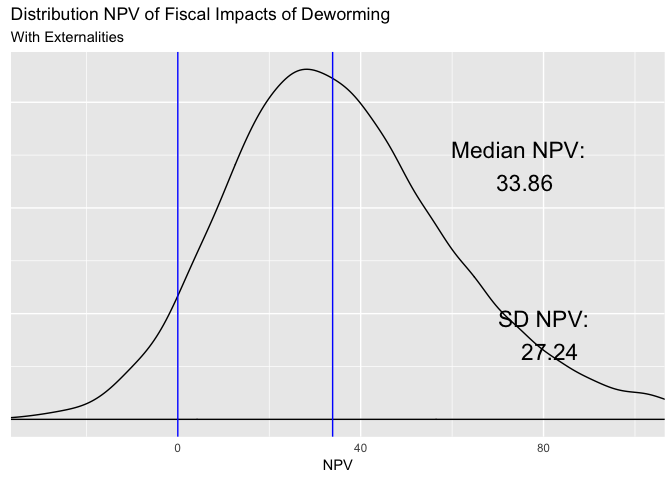
\includegraphics{03_second_opa_files/figure-latex/MC new attempt-1.pdf}

\begin{Shaded}
\begin{Highlighting}[]
\NormalTok{sim.data1 <-}\StringTok{ }\ControlFlowTok{function}\NormalTok{(}\DataTypeTok{nsims =} \FloatTok{1e4}\NormalTok{, }
\NormalTok{                      gov_bonds_vari,                }\CommentTok{#Data}
\NormalTok{                      gov_bonds_sd,}
\NormalTok{                      inflation_vari,}
\NormalTok{                      inflation_sd,}
\NormalTok{                      wage_ag_vari,}
\NormalTok{                      wage_ag_sd,}
\NormalTok{                      wage_ww_vari,}
\NormalTok{                      wage_ww_sd,}
\NormalTok{                      profits_se_vari,}
\NormalTok{                      profits_se_sd,}
\NormalTok{                      hours_se_cond_vari,}
\NormalTok{                      hours_se_cond_sd,}
\NormalTok{                      hours_ag_vari, }
\NormalTok{                      hours_ag_sd,}
\NormalTok{                      hours_ww_vari,}
\NormalTok{                      hours_ww_sd,}
\NormalTok{                      hours_se_vari,}
\NormalTok{                      hours_se_sd,}
\NormalTok{                      ex_rate_vari,}
\NormalTok{                      ex_rate_sd,}
\NormalTok{                      growth_rate_vari, }
\NormalTok{                      growth_rate_sd, }
\NormalTok{                      coverage_vari,}
\NormalTok{                      coverage_sd,}
\NormalTok{                      full_saturation_vari, }
\NormalTok{                      full_saturation_sd, }
\NormalTok{                      saturation_vari,}
\NormalTok{                      saturation_sd,}
\NormalTok{                      tax_vari, }
\NormalTok{                      tax_sd, }
\NormalTok{                      unit_cost_local_vari, }
\NormalTok{                      unit_cost_local_sd, }
\NormalTok{                      years_of_treat_vari,}
\NormalTok{                      years_of_treat_sd,}
\NormalTok{                      lambda1_vari,                   }\CommentTok{#Research}
\NormalTok{                      lambda1_sd, }
\NormalTok{                      lambda2_vari,}
\NormalTok{                      lambda2_sd,}
\NormalTok{                      q_full_vari, }
\NormalTok{                      q_full_sd,}
\NormalTok{                      q_zero_vari,}
\NormalTok{                      q_zero_sd,}
\NormalTok{                      delta_ed_par1,}
\NormalTok{                      delta_ed_sd1,}
\NormalTok{                      delta_ed_par2,}
\NormalTok{                      delta_ed_sd2,}
\NormalTok{                      coef_exp_vari,                  }\CommentTok{#Guesswork}
\NormalTok{                      coef_exp_sd,}
\NormalTok{                      teach_sal_vari,}
\NormalTok{                      teach_sal_sd,}
\NormalTok{                      teach_ben_vari,}
\NormalTok{                      teach_ben_sd,}
\NormalTok{                      n_students_vari,}
\NormalTok{                      n_students_sd, }
                      \DataTypeTok{include_ext_vari=}\OtherTok{TRUE}
\NormalTok{    ) \{}
      \KeywordTok{set.seed}\NormalTok{(}\DecValTok{1234}\NormalTok{)}
      \CommentTok{#Defaoult dist: normal, default sd: 0.1* mean}
      \CommentTok{## Data }
\NormalTok{      gov_bonds_sim <-}\StringTok{ }\KeywordTok{rnorm}\NormalTok{(}\DataTypeTok{n =}\NormalTok{ nsims, }\DataTypeTok{mean =}\NormalTok{ gov_bonds_vari, }\DataTypeTok{sd =}\NormalTok{ gov_bonds_sd)   }
\NormalTok{      inflation_sim <-}\StringTok{ }\KeywordTok{rnorm}\NormalTok{(nsims, inflation_vari, inflation_sd)}
\NormalTok{      wage_ag_sim <-}\StringTok{ }\KeywordTok{rnorm}\NormalTok{(nsims, wage_ag_vari, wage_ag_sd)}
\NormalTok{      wage_ww_sim <-}\StringTok{ }\KeywordTok{rnorm}\NormalTok{(nsims, wage_ww_vari, wage_ww_sd)}
\NormalTok{      profits_se_sim <-}\StringTok{ }\KeywordTok{rnorm}\NormalTok{(nsims, profits_se_vari, profits_se_sd)}
\NormalTok{      hours_se_cond_sim <-}\StringTok{ }\KeywordTok{rnorm}\NormalTok{(nsims, hours_se_cond_vari, hours_se_cond_sd)}
\NormalTok{      hours_ag_sim <-}\StringTok{ }\KeywordTok{rnorm}\NormalTok{(nsims, hours_ag_vari, hours_ag_sd)}
\NormalTok{      hours_ww_sim <-}\StringTok{ }\KeywordTok{rnorm}\NormalTok{(nsims, hours_ww_vari, hours_ww_sd)}
\NormalTok{      hours_se_sim <-}\StringTok{ }\KeywordTok{rnorm}\NormalTok{(nsims, hours_se_vari, hours_se_sd)}
\NormalTok{      ex_rate_sim <-}\StringTok{ }\KeywordTok{rnorm}\NormalTok{(nsims, ex_rate_vari, ex_rate_sd)}
\NormalTok{      growth_rate_sim <-}\StringTok{ }\KeywordTok{rnorm}\NormalTok{(nsims, growth_rate_vari, growth_rate_sd)}
\NormalTok{      coverage_sim <-}\StringTok{ }\KeywordTok{rnorm}\NormalTok{(nsims, coverage_vari, coverage_sd)}
\NormalTok{      saturation_sim <-}\StringTok{ }\KeywordTok{rnorm}\NormalTok{(nsims, saturation_vari, saturation_sd)}
\NormalTok{      full_saturation_sim <-}\StringTok{ }\KeywordTok{rnorm}\NormalTok{(nsims, full_saturation_vari, full_saturation_sd) }\CommentTok{###Check here later}
\NormalTok{      tax_sim <-}\StringTok{ }\KeywordTok{rnorm}\NormalTok{(nsims, tax_vari, tax_sd)}
\NormalTok{      unit_cost_local_sim <-}\StringTok{ }\KeywordTok{rnorm}\NormalTok{(nsims, unit_cost_local_vari, unit_cost_local_sd)}
\NormalTok{      years_of_treat_sim <-}\StringTok{ }\KeywordTok{rnorm}\NormalTok{(nsims, years_of_treat_vari, years_of_treat_sd)}
      
      \CommentTok{## Research}
\NormalTok{      aux1 <-}\StringTok{ }\KeywordTok{lapply}\NormalTok{(}\DecValTok{1}\OperatorTok{:}\DecValTok{2}\NormalTok{,}\ControlFlowTok{function}\NormalTok{(x) }\KeywordTok{c}\NormalTok{(lambda1_vari[x],lambda1_sd[x]) )}
\NormalTok{      lambda1_sim <-}\StringTok{ }\KeywordTok{sapply}\NormalTok{(aux1, }\ControlFlowTok{function}\NormalTok{(x)  }\KeywordTok{rnorm}\NormalTok{(nsims, }\DataTypeTok{mean =}\NormalTok{ x[}\DecValTok{1}\NormalTok{], }\DataTypeTok{sd =}\NormalTok{ x[}\DecValTok{2}\NormalTok{]) ) }
\NormalTok{      lambda2_sim <-}\StringTok{ }\KeywordTok{rnorm}\NormalTok{(nsims, lambda2_vari, lambda2_sd)}
\NormalTok{      q_full_sim <-}\StringTok{ }\KeywordTok{rnorm}\NormalTok{(nsims, q_full_vari, q_full_sd)}
\NormalTok{      q_zero_sim <-}\StringTok{ }\KeywordTok{rnorm}\NormalTok{(nsims, q_zero_vari, q_zero_sd)}
      
      \CommentTok{## Guess work}
\NormalTok{      periods_val <-}\StringTok{ }\DecValTok{50}           \CommentTok{#Total number of periods to forecast wages}
\NormalTok{      time_to_jm_val <-}\StringTok{ }\DecValTok{10}        \CommentTok{#Time from intial period until individual join the labor force}
\NormalTok{      aux2 <-}\StringTok{ }\KeywordTok{lapply}\NormalTok{(}\DecValTok{1}\OperatorTok{:}\DecValTok{2}\NormalTok{,}\ControlFlowTok{function}\NormalTok{(x) }\KeywordTok{c}\NormalTok{(coef_exp_vari[x],coef_exp_sd[x]) )}
\NormalTok{      coef_exp_val_sim <-}\StringTok{ }\KeywordTok{sapply}\NormalTok{(aux2, }\ControlFlowTok{function}\NormalTok{(x)  }\KeywordTok{rnorm}\NormalTok{(nsims, }\DataTypeTok{mean =}\NormalTok{ x[}\DecValTok{1}\NormalTok{], }\DataTypeTok{sd =}\NormalTok{ x[}\DecValTok{2}\NormalTok{]) )     }
\NormalTok{      teach_sal_val_sim <-}\StringTok{ }\KeywordTok{rnorm}\NormalTok{(nsims, teach_sal_vari, teach_sal_sd)}
\NormalTok{      teach_ben_val_sim <-}\StringTok{ }\KeywordTok{rnorm}\NormalTok{(nsims, teach_ben_vari, teach_ben_sd)}
\NormalTok{      n_students_val_sim <-}\StringTok{ }\KeywordTok{rnorm}\NormalTok{(nsims, n_students_vari, n_students_sd)}
      
\NormalTok{      delta_ed_vals_sim <-}\StringTok{ }\KeywordTok{sapply}\NormalTok{(delta_ed_so[,}\DecValTok{1}\NormalTok{], }\ControlFlowTok{function}\NormalTok{(x)  }\KeywordTok{rnorm}\NormalTok{(nsims, }\DataTypeTok{mean =} 
\NormalTok{                                                                          x }\OperatorTok{*}\StringTok{ }\NormalTok{delta_ed_par1, }
                                                                        \DataTypeTok{sd =}\NormalTok{ delta_ed_sd1 }\OperatorTok{*}\StringTok{ }\KeywordTok{sd}\NormalTok{(delta_ed_so[,}\DecValTok{1}\NormalTok{]) ) )}
      \KeywordTok{colnames}\NormalTok{(delta_ed_vals_sim) <-}\StringTok{ }\DecValTok{1999}\OperatorTok{:}\DecValTok{2007}
      
\NormalTok{      delta_ed_ext_vals_sim <-}\StringTok{ }\KeywordTok{sapply}\NormalTok{(delta_ed_ext_so[,}\DecValTok{1}\NormalTok{], }\ControlFlowTok{function}\NormalTok{(x)  }\KeywordTok{rnorm}\NormalTok{(nsims, }\DataTypeTok{mean =} 
\NormalTok{                                                                                  x }\OperatorTok{*}\StringTok{ }\NormalTok{delta_ed_par2, }
                                                                                \DataTypeTok{sd =}\NormalTok{ delta_ed_sd2 }\OperatorTok{*}\StringTok{ }\KeywordTok{sd}\NormalTok{(delta_ed_ext_so[,}\DecValTok{1}\NormalTok{])))}
      \KeywordTok{colnames}\NormalTok{(delta_ed_ext_vals_sim) <-}\StringTok{ }\DecValTok{1999}\OperatorTok{:}\DecValTok{2007}
      
\NormalTok{      track_env_var <-}\StringTok{ }\NormalTok{.GlobalEnv}

\NormalTok{      npv_sim <-}\StringTok{ }\KeywordTok{rep}\NormalTok{(}\OtherTok{NA}\NormalTok{, nsims)}
      \CommentTok{#yes externality NPV}
      \ControlFlowTok{for}\NormalTok{ (i }\ControlFlowTok{in} \DecValTok{1}\OperatorTok{:}\NormalTok{nsims) \{}
          \CommentTok{# 1 - "r""}
          \KeywordTok{invisible}\NormalTok{( }\KeywordTok{list2env}\NormalTok{( }\KeywordTok{interest_in_f}\NormalTok{(gov_bonds_sim[i], inflation_sim[i]), }\DataTypeTok{envir =}\NormalTok{ track_env_var ) )}
          \CommentTok{# 2 - "w_t"}
          \KeywordTok{invisible}\NormalTok{( }\KeywordTok{list2env}\NormalTok{( }\KeywordTok{wages_f}\NormalTok{(}\DataTypeTok{wage_ag_var_h1 =}\NormalTok{ wage_ag_sim[i],}
                                 \DataTypeTok{wage_ww_var_h =}\NormalTok{ wage_ww_sim[i],}
                                 \DataTypeTok{profits_se_var_h =}\NormalTok{ profits_se_sim[i],}
                                 \DataTypeTok{hours_se_cond_var_h =}\NormalTok{ hours_se_cond_sim[i],}
                                 \DataTypeTok{hours_ag_var_h =}\NormalTok{ hours_ag_sim[i],}
                                 \DataTypeTok{hours_ww_var_h =}\NormalTok{ hours_ww_sim[i],}
                                 \DataTypeTok{hours_se_var_h =}\NormalTok{ hours_se_sim[i],}
                                 \DataTypeTok{ex_rate_var_h =}\NormalTok{ ex_rate_sim[i], }
                                 \DataTypeTok{periods_var_h1 =}\NormalTok{ periods_so,}
                                 \DataTypeTok{time_to_jm_var_h1 =}\NormalTok{ time_to_jm_so, }
                                 \DataTypeTok{growth_rate_var_h1 =}\NormalTok{ growth_rate_sim[i],}
                                 \DataTypeTok{experience_var_h1 =}\NormalTok{ experience_temp,}
                                 \DataTypeTok{coef_exp1_var_h1 =}\NormalTok{ coef_exp_sim[i,}\DecValTok{1}\NormalTok{],}
                                 \DataTypeTok{coef_exp2_var_h1 =}\NormalTok{ coef_exp_sim[i,}\DecValTok{2}\NormalTok{]), }\DataTypeTok{envir =}\NormalTok{ track_env_var ) )}
          \CommentTok{# 3 - “λ1,γ” and “λ2,γ”}
          \KeywordTok{invisible}\NormalTok{( }\KeywordTok{list2env}\NormalTok{( }\KeywordTok{lambdas_in_f}\NormalTok{(}\DataTypeTok{lambda1_var =}\NormalTok{ lambda1_sim[i,], }\DataTypeTok{lambda2_var =}\NormalTok{ lambda2_sim[i,]), }\DataTypeTok{envir =}\NormalTok{ track_env_var) ) }
          \CommentTok{# 4 - R and p}
          \KeywordTok{invisible}\NormalTok{( }\KeywordTok{list2env}\NormalTok{(}\KeywordTok{saturation_in_f}\NormalTok{(}\DataTypeTok{coverage_var =}\NormalTok{ coverage_sim[i], }\DataTypeTok{q_full_var =}\NormalTok{ q_full_sim[i], }
                                              \DataTypeTok{q_zero_var =}\NormalTok{ q_zero_sim[i]), }\DataTypeTok{envir =}\NormalTok{ track_env_var ) )}
          \CommentTok{# 5 - K and ΔE⎯⎯⎯⎯γt(S1,S2)}
          \KeywordTok{invisible}\NormalTok{( }\KeywordTok{list2env}\NormalTok{(}\KeywordTok{ed_costs_in_f}\NormalTok{(}\DataTypeTok{teach_sal_var =}\NormalTok{ teach_sal_sim[i], }\DataTypeTok{teach_ben_var =}\NormalTok{ teach_ben_sim[i], }
                                            \DataTypeTok{n_students_var =}\NormalTok{ n_students_sim[i], }\DataTypeTok{delta_ed_ext_var =} \KeywordTok{cbind}\NormalTok{(delta_ed_ext_sim[i,], }\DecValTok{1}\NormalTok{), }
                                            \DataTypeTok{delta_ed_var =} \KeywordTok{cbind}\NormalTok{(delta_ed_sim[i,],}\DecValTok{1}\NormalTok{), }\DataTypeTok{include_ext_var =} \OtherTok{TRUE}\NormalTok{), }\DataTypeTok{envir =}\NormalTok{ track_env_var) )}
           \CommentTok{#6 - (S2Q(S2)−S1Q(S1))}
          \KeywordTok{invisible}\NormalTok{( }\KeywordTok{list2env}\NormalTok{(}\KeywordTok{costs_f}\NormalTok{(}\DataTypeTok{unit_cost_local_var =}\NormalTok{ unit_cost_local_sim[i], }\DataTypeTok{ex_rate_var =}\NormalTok{ ex_rate_sim[i], }
                                      \DataTypeTok{years_of_treat_var =}\NormalTok{ years_of_treat_sim[i], }\DataTypeTok{q_full_var =}\NormalTok{ q_full_sim[i]), }\DataTypeTok{envir =}\NormalTok{ track_env_var ) )}
          
\NormalTok{          npv_sim[i] <-}\StringTok{ }\KeywordTok{npv_mo_f}\NormalTok{(}\DataTypeTok{n_male_var =} \DecValTok{1}\OperatorTok{/}\DecValTok{2}\NormalTok{, }\DataTypeTok{n_female_var =} \DecValTok{1}\OperatorTok{/}\DecValTok{2}\NormalTok{, }
                          \DataTypeTok{interest_r_var =}\NormalTok{ interest_in,}
                          \DataTypeTok{wage_var =}\NormalTok{ wage_t_mo,}
                          \DataTypeTok{lambda1_male_var =}\NormalTok{ lambda1_in[}\DecValTok{1}\NormalTok{],}
                          \DataTypeTok{lambda1_female_var =}\NormalTok{ lambda1_in[}\DecValTok{2}\NormalTok{], }
                          \DataTypeTok{tax_var =}\NormalTok{ tax_sim[i],}
                          \DataTypeTok{saturation_var =}\NormalTok{ saturation_in,             }
                          \DataTypeTok{coverage_var =}\NormalTok{ coverage_sim[i],}
                          \DataTypeTok{cost_of_schooling_var =}\NormalTok{ cost_per_student_in,}
                          \DataTypeTok{delta_ed_male_var =}\NormalTok{ delta_ed_sim[i,],}
                          \DataTypeTok{delta_ed_female_var =}\NormalTok{ delta_ed_sim[i,], }
                          \DataTypeTok{lambda2_male_var =}\NormalTok{ lambda2_in[}\DecValTok{1}\NormalTok{],}
                          \DataTypeTok{lambda2_female_var =}\NormalTok{ lambda2_in[}\DecValTok{2}\NormalTok{],}
                          \DataTypeTok{s1_var =} \DecValTok{0}\NormalTok{, }\DataTypeTok{q1_var =} \DecValTok{0}\NormalTok{, }\DataTypeTok{s2_var =}\NormalTok{ s2_in, }\DataTypeTok{q2_var =}\NormalTok{ q2_in,}
                          \DataTypeTok{periods_var =}\NormalTok{ periods_so)}
\NormalTok{      \}}
      \KeywordTok{return}\NormalTok{(npv_sim)}
\NormalTok{    \}}





\KeywordTok{sim.data1}\NormalTok{(}\DataTypeTok{nsims =} \FloatTok{1e3}\NormalTok{, }
          \DataTypeTok{gov_bonds_vari =}\NormalTok{ gov_bonds_so, }
          \DataTypeTok{gov_bonds_sd =} \FloatTok{0.1} \OperatorTok{*}\StringTok{ }\NormalTok{gov_bonds_so,}
          \DataTypeTok{inflation_vari =}\NormalTok{ inflation_so,}
          \DataTypeTok{inflation_sd =} \FloatTok{0.1} \OperatorTok{*}\StringTok{ }\NormalTok{inflation_so,}
          \DataTypeTok{wage_ag_vari =}\NormalTok{ wage_ag_so,}
          \DataTypeTok{wage_ag_sd =} \FloatTok{0.1} \OperatorTok{*}\StringTok{ }\NormalTok{wage_ag_so,}
          \DataTypeTok{wage_ww_vari =}\NormalTok{ wage_ww_so,}
          \DataTypeTok{wage_ww_sd =} \FloatTok{0.1} \OperatorTok{*}\StringTok{ }\NormalTok{wage_ww_so,}
          \DataTypeTok{profits_se_vari =}\NormalTok{ profits_se_so, }
          \DataTypeTok{profits_se_sd =} \FloatTok{0.1} \OperatorTok{*}\StringTok{ }\NormalTok{profits_se_so, }
          \DataTypeTok{hours_se_cond_vari =}\NormalTok{ hours_se_cond_so, }
          \DataTypeTok{hours_se_cond_sd =} \FloatTok{0.1} \OperatorTok{*}\StringTok{ }\NormalTok{hours_se_cond_so, }
          \DataTypeTok{hours_ag_vari =}\NormalTok{ hours_ag_so, }
          \DataTypeTok{hours_ag_sd =} \FloatTok{0.1} \OperatorTok{*}\StringTok{ }\NormalTok{hours_ag_so, }
          \DataTypeTok{hours_ww_vari =}\NormalTok{ hours_ww_so,}
          \DataTypeTok{hours_ww_sd =} \FloatTok{0.1} \OperatorTok{*}\StringTok{ }\NormalTok{hours_ww_so,}
          \DataTypeTok{hours_se_vari =}\NormalTok{ hours_se_so,}
          \DataTypeTok{hours_se_sd =} \FloatTok{0.1} \OperatorTok{*}\StringTok{ }\NormalTok{hours_se_so,}
          \DataTypeTok{ex_rate_vari =}\NormalTok{ ex_rate_so,}
          \DataTypeTok{ex_rate_sd =} \FloatTok{0.1} \OperatorTok{*}\StringTok{ }\NormalTok{ex_rate_so,}
          \DataTypeTok{growth_rate_vari =}\NormalTok{ growth_rate_so,}
          \DataTypeTok{growth_rate_sd =} \FloatTok{0.1} \OperatorTok{*}\StringTok{ }\NormalTok{growth_rate_so,}
          \DataTypeTok{coverage_vari =}\NormalTok{ coverage_so,}
          \DataTypeTok{coverage_sd =} \FloatTok{0.1} \OperatorTok{*}\StringTok{ }\NormalTok{coverage_so,}
          \DataTypeTok{saturation_vari =} \DecValTok{1}\NormalTok{,}
          \DataTypeTok{saturation_sd =} \DecValTok{1}\NormalTok{,}
          \DataTypeTok{tax_vari =}\NormalTok{ tax_so, }
          \DataTypeTok{tax_sd =} \FloatTok{0.1} \OperatorTok{*}\StringTok{ }\NormalTok{tax_so, }
          \DataTypeTok{unit_cost_local_vari =}\NormalTok{ unit_cost_local_so, }
          \DataTypeTok{unit_cost_local_sd =} \FloatTok{0.1} \OperatorTok{*}\StringTok{ }\NormalTok{unit_cost_local_so, }
          \DataTypeTok{years_of_treat_vari =}\NormalTok{ years_of_treat_so,}
          \DataTypeTok{years_of_treat_sd =} \FloatTok{0.1} \OperatorTok{*}\StringTok{ }\NormalTok{years_of_treat_so,}
          \DataTypeTok{lambda1_vari =}\NormalTok{ lambda1_so,}
          \DataTypeTok{lambda1_sd =} \FloatTok{0.1} \OperatorTok{*}\StringTok{ }\KeywordTok{c}\NormalTok{(lambda1_so[}\DecValTok{1}\NormalTok{], }\FloatTok{0.01}\NormalTok{),}
          \DataTypeTok{lambda2_vari =}\NormalTok{ lambda2_so, }
          \DataTypeTok{lambda2_sd =} \FloatTok{0.1} \OperatorTok{*}\StringTok{ }\NormalTok{lambda2_so, }
          \DataTypeTok{q_full_vari =}\NormalTok{ q_full_so, }
          \DataTypeTok{q_full_sd =} \FloatTok{0.1} \OperatorTok{*}\StringTok{ }\NormalTok{q_full_so, }
          \DataTypeTok{q_zero_vari =}\NormalTok{ q_zero_so, }
          \DataTypeTok{q_zero_sd =} \FloatTok{0.1} \OperatorTok{*}\StringTok{ }\NormalTok{q_zero_so, }
          \DataTypeTok{coef_exp_vari =}\NormalTok{ coef_exp_so, }
          \DataTypeTok{coef_exp_sd =} \KeywordTok{c}\NormalTok{(}\FloatTok{0.001}\NormalTok{ , }\FloatTok{0.001}\NormalTok{), }
          \DataTypeTok{teach_sal_vari =}\NormalTok{ teach_sal_so,}
          \DataTypeTok{teach_sal_sd =} \FloatTok{0.1} \OperatorTok{*}\StringTok{ }\NormalTok{teach_sal_so,}
          \DataTypeTok{teach_ben_vari =}\NormalTok{ teach_ben_so,}
          \DataTypeTok{teach_ben_sd =} \FloatTok{0.1} \OperatorTok{*}\StringTok{ }\NormalTok{teach_ben_so,}
          \DataTypeTok{n_students_vari =}\NormalTok{ n_students_so, }
          \DataTypeTok{n_students_sd =} \FloatTok{0.1} \OperatorTok{*}\StringTok{ }\NormalTok{n_students_so, }
          \DataTypeTok{include_ext_vari =} \OtherTok{TRUE}\NormalTok{, }
          \DataTypeTok{full_saturation_vari =}\NormalTok{ full_saturation_so,}
          \DataTypeTok{full_saturation_sd =} \FloatTok{0.1} \OperatorTok{*}\StringTok{ }\NormalTok{full_saturation_so,}
          \DataTypeTok{delta_ed_par1 =} \DecValTok{1}\NormalTok{,}
          \DataTypeTok{delta_ed_sd1 =} \DecValTok{1}\NormalTok{,}
          \DataTypeTok{delta_ed_par2 =} \DecValTok{1}\NormalTok{,}
          \DataTypeTok{delta_ed_sd2 =} \DecValTok{1}
\NormalTok{) }
 
 




\CommentTok{# run the model }
\CommentTok{#  input: Input vectors for NPV function}
\CommentTok{#  output: one vector of NPVs (of lenght Nsims)}
\CommentTok{# Repeat Nsims times}
\CommentTok{#  input: all functions from above + NSims}
\CommentTok{#  output: vector of Results of length NSims}

\CommentTok{# TO DO: fix negative wage trends do to high negative term in the square of experience. }

\CommentTok{#  generate 1 draw of primitive values:}
\CommentTok{#  inputs: K primitive means and K standard deviations}
\CommentTok{#  output: K values with one from simulations}

\CommentTok{# asd <- one_draw()}
\CommentTok{# Takes each element of list and assings it an object with the same name}
\CommentTok{# list2env(asd,.GlobalEnv)}
\CommentTok{# compute the elements of the model}
\CommentTok{#  input: K vectors with draws from sims}
\CommentTok{#  output: Input vectors for NPV functions}
\end{Highlighting}
\end{Shaded}

\begin{Shaded}
\begin{Highlighting}[]
\CommentTok{# -0.6096942}
\NormalTok{sims_f <-}\StringTok{ }\ControlFlowTok{function}\NormalTok{(..., }\DataTypeTok{n_sims_var =} \DecValTok{10}\NormalTok{) \{}
\NormalTok{track_env_var <-}\StringTok{ }\NormalTok{.GlobalEnv}

\NormalTok{    npv_sim <-}\StringTok{ }\KeywordTok{rep}\NormalTok{(}\OtherTok{NA}\NormalTok{, n_sims_var)}
    \ControlFlowTok{for}\NormalTok{ (i }\ControlFlowTok{in} \DecValTok{1}\OperatorTok{:}\NormalTok{n_sims_var) \{}
    \CommentTok{#if (i>=2) \{rm(ls(pattern = "_sim\textbackslash{}\textbackslash{}b"))\}}
    \CommentTok{#rm(list = ls()[!(ls() %in% (ls(pattern = "_so\textbackslash{}\textbackslash{}b") )])}
    \KeywordTok{invisible}\NormalTok{( }\KeywordTok{list2env}\NormalTok{(}\KeywordTok{onedraw_sim_f}\NormalTok{(...), }\DataTypeTok{envir =}\NormalTok{ track_env_var ) )}
    \CommentTok{# 1 - "r""}
    \KeywordTok{invisible}\NormalTok{( }\KeywordTok{list2env}\NormalTok{( }\KeywordTok{interest_in_f}\NormalTok{(gov_bonds_sim, inflation_sim), }\DataTypeTok{envir =}\NormalTok{ track_env_var ) )}
    \CommentTok{# 2 - "w_t"}
    \KeywordTok{invisible}\NormalTok{( }\KeywordTok{list2env}\NormalTok{( }\KeywordTok{wages_f}\NormalTok{(}\DataTypeTok{wage_ag_var_h1 =}\NormalTok{ wage_ag_sim,}
                           \DataTypeTok{wage_ww_var_h =}\NormalTok{ wage_ww_sim,}
                           \DataTypeTok{profits_se_var_h =}\NormalTok{ profits_se_sim,}
                           \DataTypeTok{hours_se_cond_var_h =}\NormalTok{ hours_se_cond_sim,}
                           \DataTypeTok{hours_ag_var_h =}\NormalTok{ hours_ag_sim,}
                           \DataTypeTok{hours_ww_var_h =}\NormalTok{ hours_ww_sim,}
                           \DataTypeTok{hours_se_var_h =}\NormalTok{ hours_se_sim,}
                           \DataTypeTok{ex_rate_var_h =}\NormalTok{ ex_rate_sim, }
                           \DataTypeTok{periods_var_h1 =}\NormalTok{ periods_so,}
                           \DataTypeTok{time_to_jm_var_h1 =}\NormalTok{ time_to_jm_so, }
                           \DataTypeTok{growth_rate_var_h1 =}\NormalTok{ growth_rate_sim,}
                           \DataTypeTok{experience_var_h1 =}\NormalTok{ experience_temp,}
                           \DataTypeTok{coef_exp1_var_h1 =}\NormalTok{ coef_exp_sim[}\DecValTok{1}\NormalTok{],}
                           \DataTypeTok{coef_exp2_var_h1 =}\NormalTok{ coef_exp_sim[}\DecValTok{2}\NormalTok{]), }\DataTypeTok{envir =}\NormalTok{ track_env_var ) )}
    \CommentTok{# 3 - “λ1,γ” and “λ2,γ”}
    \KeywordTok{invisible}\NormalTok{( }\KeywordTok{list2env}\NormalTok{( }\KeywordTok{lambdas_in_f}\NormalTok{(}\DataTypeTok{lambda1_var =}\NormalTok{ lambda1_sim, }\DataTypeTok{lambda2_var =}\NormalTok{ lambda2_sim), }\DataTypeTok{envir =}\NormalTok{ track_env_var) ) }
    \CommentTok{# 4 - R and p}
    \KeywordTok{invisible}\NormalTok{( }\KeywordTok{list2env}\NormalTok{(}\KeywordTok{saturation_in_f}\NormalTok{(}\DataTypeTok{coverage_var =}\NormalTok{ coverage_sim, }\DataTypeTok{q_full_var =}\NormalTok{ q_full_sim, }
                                        \DataTypeTok{q_zero_var =}\NormalTok{ q_zero_sim), }\DataTypeTok{envir =}\NormalTok{ track_env_var ) )}
    \CommentTok{# 5 - K and ΔE⎯⎯⎯⎯γt(S1,S2)}
    \KeywordTok{invisible}\NormalTok{( }\KeywordTok{list2env}\NormalTok{(}\KeywordTok{ed_costs_in_f}\NormalTok{(}\DataTypeTok{teach_sal_var =}\NormalTok{ teach_sal_sim, }\DataTypeTok{teach_ben_var =}\NormalTok{ teach_ben_sim, }
                                      \DataTypeTok{n_students_var =}\NormalTok{ n_students_sim, }\DataTypeTok{delta_ed_ext_var =} \KeywordTok{cbind}\NormalTok{(delta_ed_ext_sim, }\DecValTok{1}\NormalTok{), }
                                      \DataTypeTok{delta_ed_var =} \KeywordTok{cbind}\NormalTok{(delta_ed_sim,}\DecValTok{1}\NormalTok{), }\DataTypeTok{include_ext_var =} \OtherTok{TRUE}\NormalTok{), }\DataTypeTok{envir =}\NormalTok{ track_env_var) )}
     \CommentTok{#6 - (S2Q(S2)−S1Q(S1))}
    \KeywordTok{invisible}\NormalTok{( }\KeywordTok{list2env}\NormalTok{(}\KeywordTok{costs_f}\NormalTok{(}\DataTypeTok{unit_cost_local_var =}\NormalTok{ unit_cost_local_sim, }\DataTypeTok{ex_rate_var =}\NormalTok{ ex_rate_sim, }
                                \DataTypeTok{years_of_treat_var =}\NormalTok{ years_of_treat_sim, }\DataTypeTok{q_full_var =}\NormalTok{ q_full_sim), }\DataTypeTok{envir =}\NormalTok{ track_env_var ) )}
    
\NormalTok{    npv_sim[i] <-}\StringTok{ }\KeywordTok{npv_mo_f}\NormalTok{(}\DataTypeTok{n_male_var =} \DecValTok{1}\OperatorTok{/}\DecValTok{2}\NormalTok{, }\DataTypeTok{n_female_var =} \DecValTok{1}\OperatorTok{/}\DecValTok{2}\NormalTok{, }
                    \DataTypeTok{interest_r_var =}\NormalTok{ interest_in,}
                    \DataTypeTok{wage_var =}\NormalTok{ wage_t_mo,}
                    \DataTypeTok{lambda1_male_var =}\NormalTok{ lambda1_in[}\DecValTok{1}\NormalTok{],}
                    \DataTypeTok{lambda1_female_var =}\NormalTok{ lambda1_in[}\DecValTok{2}\NormalTok{], }
                    \DataTypeTok{tax_var =}\NormalTok{ tax_sim,}
                    \DataTypeTok{saturation_var =}\NormalTok{ saturation_in,             }
                    \DataTypeTok{coverage_var =}\NormalTok{ coverage_sim,}
                    \DataTypeTok{cost_of_schooling_var =}\NormalTok{ cost_per_student_in,}
                    \DataTypeTok{delta_ed_male_var =}\NormalTok{ delta_ed_sim,}
                    \DataTypeTok{delta_ed_female_var =}\NormalTok{ delta_ed_sim, }
                    \DataTypeTok{lambda2_male_var =}\NormalTok{ lambda2_in[}\DecValTok{1}\NormalTok{],}
                    \DataTypeTok{lambda2_female_var =}\NormalTok{ lambda2_in[}\DecValTok{2}\NormalTok{],}
                    \DataTypeTok{s1_var =} \DecValTok{0}\NormalTok{, }\DataTypeTok{q1_var =} \DecValTok{0}\NormalTok{, }\DataTypeTok{s2_var =}\NormalTok{ s2_in, }\DataTypeTok{q2_var =}\NormalTok{ q2_in,}
                    \DataTypeTok{periods_var =}\NormalTok{ periods_so)}
    \CommentTok{#if (npv_sim[i]<0) \{browser()\}}
\NormalTok{    \}}
    \KeywordTok{return}\NormalTok{(npv_sim)}
\NormalTok{\}}
\end{Highlighting}
\end{Shaded}

\begin{Shaded}
\begin{Highlighting}[]
\KeywordTok{rm}\NormalTok{(}\DataTypeTok{list =} \KeywordTok{ls}\NormalTok{()[}\OperatorTok{!}\NormalTok{(}\KeywordTok{ls}\NormalTok{() }\OperatorTok\StringTok{ }\KeywordTok{ls}\NormalTok{(}\DataTypeTok{pattern =} \StringTok{"_f}\CharTok{\textbackslash{}\textbackslash{}}\StringTok{b"}\NormalTok{) )])}

\KeywordTok{set.seed}\NormalTok{(}\DecValTok{142857}\NormalTok{)}

\KeywordTok{invisible}\NormalTok{( }\KeywordTok{list2env}\NormalTok{(}\KeywordTok{call_params_f}\NormalTok{(), .GlobalEnv) )}

\NormalTok{track_env <-}\StringTok{ }\KeywordTok{environment}\NormalTok{()}


\NormalTok{npv_sim <-}\StringTok{ }\KeywordTok{sims_f}\NormalTok{(}\DataTypeTok{n_sims_var =} \FloatTok{1e4}\NormalTok{)}

\CommentTok{########}
\CommentTok{# ANALYSE OUTPUT}

\CommentTok{# unit test}
\ControlFlowTok{if}\NormalTok{ (}\KeywordTok{abs}\NormalTok{(}\KeywordTok{sd}\NormalTok{(npv_sim) }\OperatorTok{-}\StringTok{ }\FloatTok{28.38155}\NormalTok{)}\OperatorTok{>}\FloatTok{0.0001}\NormalTok{ ) \{}
  \KeywordTok{print}\NormalTok{(}\StringTok{"Output has change"}\NormalTok{)}
\NormalTok{\}}

\NormalTok{npv_for_text <-}\StringTok{ }\KeywordTok{paste}\NormalTok{(}\StringTok{"Median NPV:}\CharTok{\textbackslash{}n}\StringTok{ "}\NormalTok{, }\KeywordTok{round}\NormalTok{(}\KeywordTok{median}\NormalTok{(npv_sim), }\DecValTok{2}\NormalTok{))}
\NormalTok{npv_for_text2 <-}\StringTok{ }\KeywordTok{paste}\NormalTok{(}\StringTok{"SD NPV:}\CharTok{\textbackslash{}n}\StringTok{ "}\NormalTok{, }\KeywordTok{round}\NormalTok{(}\KeywordTok{sd}\NormalTok{(npv_sim), }\DecValTok{2}\NormalTok{))}

\KeywordTok{ggplot}\NormalTok{() }\OperatorTok{+}
\StringTok{  }\KeywordTok{geom_density}\NormalTok{(}\KeywordTok{aes}\NormalTok{(}\DataTypeTok{x =}\NormalTok{ npv_sim,}
                   \DataTypeTok{alpha =} \DecValTok{1}\OperatorTok{/}\DecValTok{2}\NormalTok{), }\DataTypeTok{kernel =} \StringTok{"gau"}\NormalTok{) }\OperatorTok{+}
\StringTok{  }\KeywordTok{geom_vline}\NormalTok{(}\DataTypeTok{xintercept =} \KeywordTok{c}\NormalTok{(}\DecValTok{0}\NormalTok{, }\KeywordTok{median}\NormalTok{(npv_sim)), }\DataTypeTok{col=}\StringTok{"blue"}\NormalTok{) }\OperatorTok{+}
\StringTok{  }\KeywordTok{coord_cartesian}\NormalTok{(}\DataTypeTok{xlim =} \KeywordTok{c}\NormalTok{(}\OperatorTok{-}\DecValTok{30}\NormalTok{,}\DecValTok{100}\NormalTok{)) }\OperatorTok{+}
\StringTok{  }\KeywordTok{guides}\NormalTok{(}\DataTypeTok{alpha =} \StringTok{"none"}\NormalTok{, }\DataTypeTok{colour=}\StringTok{"none"}\NormalTok{) }\OperatorTok{+}
\StringTok{  }\KeywordTok{labs}\NormalTok{(}\DataTypeTok{y =} \OtherTok{NULL}\NormalTok{,}
       \DataTypeTok{x =} \StringTok{"NPV"}\NormalTok{ ,}
       \DataTypeTok{title =} \StringTok{"Distribution NPV of Fiscal Impacts of Deworming"}\NormalTok{,}
       \DataTypeTok{subtitle =} \StringTok{"With Externalities"}\NormalTok{)}\OperatorTok{+}
\StringTok{  }\KeywordTok{annotate}\NormalTok{(}\StringTok{"text"}\NormalTok{, }\DataTypeTok{x =} \FloatTok{2.2} \OperatorTok{*}\StringTok{ }\KeywordTok{median}\NormalTok{(npv_sim), }\DataTypeTok{y =} \FloatTok{0.012}\NormalTok{, }\DataTypeTok{label =}\NormalTok{ npv_for_text, }\DataTypeTok{size =} \DecValTok{6}\NormalTok{)}\OperatorTok{+}
\StringTok{  }\KeywordTok{annotate}\NormalTok{(}\StringTok{"text"}\NormalTok{, }\DataTypeTok{x =} \DecValTok{80}\NormalTok{, }\DataTypeTok{y =} \FloatTok{0.004}\NormalTok{, }\DataTypeTok{label =}\NormalTok{ npv_for_text2, }\DataTypeTok{size =} \DecValTok{6}\NormalTok{)}\OperatorTok{+}
\StringTok{  }\KeywordTok{theme}\NormalTok{(}\DataTypeTok{axis.ticks =} \KeywordTok{element_blank}\NormalTok{(), }\DataTypeTok{axis.text.y =} \KeywordTok{element_blank}\NormalTok{())}
\end{Highlighting}
\end{Shaded}

\begin{Shaded}
\begin{Highlighting}[]
\KeywordTok{rm}\NormalTok{(}\DataTypeTok{list =} \KeywordTok{ls}\NormalTok{()[}\OperatorTok{!}\NormalTok{(}\KeywordTok{ls}\NormalTok{() }\OperatorTok\StringTok{ }\KeywordTok{ls}\NormalTok{(}\DataTypeTok{pattern =} \StringTok{"_f}\CharTok{\textbackslash{}\textbackslash{}}\StringTok{b"}\NormalTok{) )])}


\KeywordTok{list2env}\NormalTok{(}\KeywordTok{call_params_f}\NormalTok{(), .GlobalEnv)}

    \CommentTok{#rm(list = ls(pattern= "_so\textbackslash{}\textbackslash{}b") )}
 
    \CommentTok{#invisible( list2env(onedraw_sim_f(), .GlobalEnv ) )}
    \CommentTok{# 1 - "r""}
    \KeywordTok{invisible}\NormalTok{( }\KeywordTok{list2env}\NormalTok{( }\KeywordTok{interest_in_f}\NormalTok{(gov_bonds_so, inflation_so), .GlobalEnv ) )}
    \CommentTok{# 2 - "w_t"}
    \KeywordTok{invisible}\NormalTok{( }\KeywordTok{list2env}\NormalTok{( }\KeywordTok{wages_f}\NormalTok{(}\DataTypeTok{wage_ag_var_h1 =}\NormalTok{ wage_ag_so,}
                           \DataTypeTok{wage_ww_var_h =}\NormalTok{ wage_ww_so,}
                           \DataTypeTok{profits_se_var_h =}\NormalTok{ profits_se_so,}
                           \DataTypeTok{hours_se_cond_var_h =}\NormalTok{ hours_se_cond_so,}
                           \DataTypeTok{hours_ag_var_h =}\NormalTok{ hours_ag_so,}
                           \DataTypeTok{hours_ww_var_h =}\NormalTok{ hours_ww_so,}
                           \DataTypeTok{hours_se_var_h =}\NormalTok{ hours_se_so,}
                           \DataTypeTok{ex_rate_var_h =}\NormalTok{ ex_rate_so, }
                           \DataTypeTok{periods_var_h1 =}\NormalTok{ periods_so,}
                           \DataTypeTok{time_to_jm_var_h1 =}\NormalTok{ time_to_jm_so, }
                           \DataTypeTok{growth_rate_var_h1 =}\NormalTok{ growth_rate_so,}
                           \DataTypeTok{experience_var_h1 =}\NormalTok{ experience_temp,}
                           \DataTypeTok{coef_exp1_var_h1 =}\NormalTok{ coef_exp_so[}\DecValTok{1}\NormalTok{],}
                           \DataTypeTok{coef_exp2_var_h1 =}\NormalTok{ coef_exp_so[}\DecValTok{2}\NormalTok{]), .GlobalEnv ) )}
    \CommentTok{# 3 - “λ1,γ” and “λ2,γ”}
    \KeywordTok{invisible}\NormalTok{( }\KeywordTok{list2env}\NormalTok{( }\KeywordTok{lambdas_in_f}\NormalTok{(}\DataTypeTok{lambda1_var =}\NormalTok{ lambda1_so, }\DataTypeTok{lambda2_var =}\NormalTok{ lambda2_so), .GlobalEnv ) ) }
    \CommentTok{# 4 - R and p}
    \KeywordTok{invisible}\NormalTok{( }\KeywordTok{list2env}\NormalTok{(}\KeywordTok{saturation_in_f}\NormalTok{(}\DataTypeTok{coverage_var =}\NormalTok{ coverage_so, }\DataTypeTok{q_full_var =}\NormalTok{ q_full_so, }
                                        \DataTypeTok{q_zero_var =}\NormalTok{ q_zero_so), .GlobalEnv ) )}
    \CommentTok{# 5 - K and ΔE⎯⎯⎯⎯γt(S1,S2)}
    \KeywordTok{invisible}\NormalTok{( }\KeywordTok{list2env}\NormalTok{(}\KeywordTok{ed_costs_in_f}\NormalTok{(}\DataTypeTok{teach_sal_var =}\NormalTok{ teach_sal_so, }\DataTypeTok{teach_ben_var =}\NormalTok{ teach_ben_so, }
                                      \DataTypeTok{n_students_var =}\NormalTok{ n_students_so, }\DataTypeTok{delta_ed_ext_var =}\NormalTok{ delta_ed_ext_so, }
                                      \DataTypeTok{delta_ed_var =}\NormalTok{ delta_ed_so, }\DataTypeTok{include_ext_var =} \OtherTok{TRUE}\NormalTok{), .GlobalEnv ) )}
     \CommentTok{#6 - (S2Q(S2)−S1Q(S1))}
    \KeywordTok{invisible}\NormalTok{( }\KeywordTok{list2env}\NormalTok{(}\KeywordTok{costs_f}\NormalTok{(}\DataTypeTok{unit_cost_local_var =}\NormalTok{ unit_cost_local_so, }\DataTypeTok{ex_rate_var =}\NormalTok{ ex_rate_so, }
                                \DataTypeTok{years_of_treat_var =}\NormalTok{ years_of_treat_so, }\DataTypeTok{q_full_var =}\NormalTok{ q_full_so), .GlobalEnv ) )}
    
    \KeywordTok{npv_mo_f}\NormalTok{(}\DataTypeTok{n_male_var =} \DecValTok{1}\OperatorTok{/}\DecValTok{2}\NormalTok{, }\DataTypeTok{n_female_var =} \DecValTok{1}\OperatorTok{/}\DecValTok{2}\NormalTok{, }
                    \DataTypeTok{interest_r_var =}\NormalTok{ interest_in,}
                    \DataTypeTok{wage_var =}\NormalTok{ wage_t_mo,}
                    \DataTypeTok{lambda1_male_var =}\NormalTok{ lambda1_in[}\DecValTok{1}\NormalTok{],}
                    \DataTypeTok{lambda1_female_var =}\NormalTok{ lambda1_in[}\DecValTok{2}\NormalTok{], }
                    \DataTypeTok{tax_var =}\NormalTok{ tax_so,}
                    \DataTypeTok{saturation_var =}\NormalTok{ saturation_in,             }
                    \DataTypeTok{coverage_var =}\NormalTok{ coverage_so,}
                    \DataTypeTok{cost_of_schooling_var =}\NormalTok{ cost_per_student_in,}
                    \DataTypeTok{delta_ed_male_var =}\NormalTok{ delta_ed_so[,}\DecValTok{1}\NormalTok{],}
                    \DataTypeTok{delta_ed_female_var =}\NormalTok{ delta_ed_so[,}\DecValTok{1}\NormalTok{], }
                    \DataTypeTok{lambda2_male_var =} \DecValTok{0}\NormalTok{,}
                    \DataTypeTok{lambda2_female_var =} \DecValTok{0}\NormalTok{,}
                    \DataTypeTok{s1_var =} \DecValTok{0}\NormalTok{, }\DataTypeTok{q1_var =} \DecValTok{0}\NormalTok{, }\DataTypeTok{s2_var =}\NormalTok{ s2_in, }\DataTypeTok{q2_var =}\NormalTok{ q2_in,}
                    \DataTypeTok{periods_var =}\NormalTok{ periods_so)}
\end{Highlighting}
\end{Shaded}

\hypertarget{sensitivity-analysis}{%
\section{Sensitivity Analysis}\label{sensitivity-analysis}}


\end{document}
